\documentclass[11pt]{article}

\usepackage[a4paper, margin=2.5cm]{geometry}
\usepackage{amsmath, amssymb, amsthm}
\usepackage{booktabs}
\usepackage{enumitem}
\usepackage{graphicx}
\usepackage{natbib}
\usepackage[colorlinks=true, linkcolor=blue, citecolor=blue, urlcolor=blue]{hyperref}
\usepackage{xcolor}

\graphicspath{{figures/}{../reports/figures/}}

\title{A geometry-derived response kernel for the\\
       $B \to K^{*}\mu^{+}\mu^{-}$ angular anomaly:\\
       sign-uniform cross-dataset and cross-channel fit}

\author{%
  Lee Smart\\[2pt]
  \textit{Institute of Vibrational Field Dynamics}\\[2pt]
  \texttt{contact@vibrationalfielddynamics.org}\\[2pt]
  \texttt{@vfd\_org}%
}

\date{April 2026}

\begin{document}

\maketitle

\noindent\textbf{Status:} Preprint, not peer-reviewed.

\noindent\emph{Negative-of-headline result.}
A fully non-linear refit
(\texttt{flavio.\allowbreak np\_\allowbreak prediction})
shows the geometry-derived kernel is statistically
indistinguishable from a constant $\Delta C_{9}$ shift on AIC.
An earlier linearised analysis (Mode B) had found a marginal
preference for the kernel that did not survive the non-linear test.
The remaining structural finding is direction consistency of the
fitted amplitude across two collaborations, three decay channels,
and five fits — a property that follows from any sufficiently
centre-peaked one-parameter shape on the same anomaly and which the
geometric kernel satisfies but does not uniquely deliver.

\begin{abstract}
We test whether a single $q^{2}$-dependent response kernel
$\kappa(q^{2})$, constructed from a finite 2I-equivariant graph
substrate (the 600-cell $V_{600}$) regularised by the golden ratio
$\varphi$ as a discrete mass scale, can describe the
$B^{0}\to K^{*0}\mu^{+}\mu^{-}$ angular anomaly across multiple
datasets and decay channels. The kernel is the shell-mean
projection of the discrete Green's response
$\psi = (L_{V_{600}} + \varphi^{-2} I)^{-1} f$, with $f$ a uniform
source on the equatorial inner-product shell; the kernel shape has no
continuous fitted parameters. The continuum limit is
$\kappa(x) = e^{-|x|/\varphi}$ with
$x = (q^{2}-q^{2}_{\mathrm{mid}})/\Delta_{\psi}$, where
$q^{2}_{\mathrm{mid}}$ and $\Delta_{\psi}$ are the
$J/\psi$\,-\,$\psi(2S)$ midpoint and half-spread. Of three discrete
edge-weighting variants the unweighted Laplacian is selected; we show
in \S\ref{sec:derivation} that this same variant wins on a
pure-geometry criterion (correlation with the continuum kernel)
independent of the LHCb data.

Using \texttt{flavio}~\citep{Straub2018Flavio} for SM and
non-linear-in-$C_{9}$ predictions on each dataset's own bin
grid, and fitting only one dimensionless amplitude $A$ per dataset, we
find:
(i) on the LHCb 2025 data~\citep{LHCb2025BKstmumuComp} the kernel
gives $\Delta\mathrm{AIC}=+1.09$ vs a free $\Delta C_{9}$ shift on a
joint fit of four angular observables (P5', P4', P1, P2): a marginal
\emph{disfavouring} of the kernel relative to the constant shift, both
at $k=1$;
(ii) on five fits across two collaborations and three decay channels
— LHCb~2015~\citep{LHCb2015BKstmumu},
LHCb~2021 ($B^{+}\!\to\!K^{*+}$)~\citep{LHCb2021BKstpmumu},
CMS~2025~\citep{CMS2025BKstmumu}, LHCb~2025, and
$B_{s}\!\to\!\phi\mu\mu$~\citep{LHCb2015Bsphimumu} — the
non-linear $\Delta\mathrm{AIC}$ values span $[-0.24, +1.09]$ around
zero, with $2/5$ datasets favouring the kernel and $3/5$ favouring
the constant shift; the stacked Akaike weight is
$w_{\mathrm{VFD}}=0.35$ vs $w_{\mathrm{FREE\_C9}}=0.65$;
(iii) the fitted amplitudes are sign-uniform across all five fits
($A>0$ in every fit, effective $\Delta C_{9}^{\mathrm{eff}}<0$ in
every fit); the null against which this is non-trivial is the
``no anomaly'' null, against which $\mathrm{FREE\_C9}$ would also
produce $5/5$ same-sign fits — sign-uniformity confirms the kernel
is consistent in direction with the established anomaly, not that
the kernel is preferred over a constant Wilson-coefficient shift;
(iv) the apparent factor-of-3 amplitude difference between the
$P$-basis $B\to K^{*}$ fits and the $S$-basis $B_{s}\!\to\!\phi$ fit
is mostly a basis effect (Krüger--Matias $P_{i}$ vs CP-averaged
$S_{i}$), with a residual $\sim 50\,\%$ overshoot of the
basis-corrected prediction that we cannot resolve given the published
2015 $B_{s}\!\to\!\phi$ statistics and the absence of an angular
covariance matrix.

The kernel is consistent with the angular anomaly's $q^{2}$ shape but
does not improve over a constant Wilson-coefficient shift on AIC under
non-linear evaluation. The surviving claim is direction-consistency
across two collaborations, three decay channels, and five fits, with
no per-dataset shape retuning — a claim that follows from any
sufficiently centre-peaked single-parameter shape on the same anomaly,
and which the geometric kernel satisfies but does not uniquely
deliver. We do not claim the kernel is the preferred or unique shape:
a free-width Gaussian charm-loop proxy fits marginally better in
$\chi^{2}$ at the cost of one extra parameter. A previous linearised
analysis (linear in $\Delta C_{9}$ via central-difference slopes)
found a stronger result that did not survive the non-linear refit;
the earlier numbers are reproduced as a linearisation diagnostic in
\S\ref{sec:method}.
\end{abstract}

% =====================================================================
% =====================================================================
\section{Introduction}\label{sec:intro}
% =====================================================================

The angular distribution of the rare flavour-changing-neutral-current
decay $B^{0}\to K^{*0}\mu^{+}\mu^{-}$ has shown a persistent tension
with Standard-Model predictions for over a decade, conventionally
parametrised as a negative shift in the semileptonic vector Wilson
coefficient $\Delta C_{9}\sim -1$ relative to the SM benchmark
$C_{9}^{\mathrm{SM}}\approx 4.27$
\citep{Descotes2013P5p,AltmannshoferStraub2013}. The most recent LHCb
comprehensive analysis \citep{LHCb2025BKstmumuComp,LHCb2025BKstmumuHEPData}
confirms the pattern at $8.4\,\mathrm{fb}^{-1}$, with full angular and
branching-fraction observables determined on the same dataset.

Free Wilson-coefficient fits have served as the standard interpretive
ansatz: one fits a constant shift $\Delta C_{9}$ across all $q^{2}$ bins
and reports the best-fit value and its uncertainty. The free shift makes
no commitment to the underlying shape of any new-physics effect: by
construction it averages over all bins with weight inversely proportional
to the squared sensitivity. If the underlying physics has a non-trivial
$q^{2}$ dependence — for example, a centre-peaked structure between the
charmonium resonances, or an oscillation with a definite scale — that
information is discarded.

This paper asks a deliberately constrained question. Suppose the
$q^{2}$-dependent response kernel $\kappa(q^{2})$ is fixed
\emph{a priori} by an external geometric construction, with no shape
parameters tunable to the data, and one fits only its overall
amplitude. Does the same kernel describe multiple datasets and channels
with no per-dataset retuning?

Concretely, we take $\kappa(q^{2})$ to be the discrete Green's response
of a finite 2I-equivariant graph (the 600-cell $V_{600}$, vertices and
edges of the regular 4-polytope) regularised by the golden ratio
$\varphi=(1+\sqrt{5})/2$ as a discrete mass scale,
\begin{equation}\label{eq:kernel_def}
\psi = \bigl(L_{V_{600}} + \varphi^{-2}\, I\bigr)^{-1} f,
\qquad
\kappa(q^{2}) = \mathrm{shell\text{-}mean}\!\bigl[\psi\bigr]\!\Bigl(x(q^{2})\Bigr),
\end{equation}
with $f$ a uniform source on the equatorial inner-product shell,
$L_{V_{600}}$ the standard graph Laplacian, and $x(q^{2}) =
(q^{2}-q^{2}_{\mathrm{mid}})/\Delta_{\psi}$ a dimensionless coordinate
anchored at the $J/\psi$\,--\,$\psi(2S)$ midpoint. The construction is
motivated by the substrate spectral framework of the companion VFD
preprints \citep{SmartCrystallisation2026,SmartAdaptiveClosureTransport2026};
its derivation as the appropriate object for compressing this anomaly
is given in section~\ref{sec:derivation}. The continuum limit is the
exponential $\kappa(x) = e^{-|x|/\varphi}$. No shape parameter is
fitted to any dataset.

The fit form everywhere in this paper is
\begin{equation}\label{eq:fit_form}
\Delta C_{9}^{\mathrm{VFD}}(q^{2}) \;=\; -A\,\kappa(q^{2}),
\end{equation}
with $A$ the only fitted parameter. The kernel is identical across
every dataset and decay channel; SM predictions and Wilson-coefficient
slopes are regenerated per dataset on its own $q^{2}$ bin grid using
\texttt{flavio} 2.4 \citep{Straub2018Flavio}.

\subsection*{Scope and epistemic status}

This paper reports two analyses of the same data: a linearised fit
(Mode~B; first-order Taylor expansion of every angular observable
in $\Delta C_{9}$ around $C_{9}^{\mathrm{SM}}$) and a fully
non-linear fit using \texttt{flavio.np\_prediction} directly. The
fitted $\Delta C_{9}$ values are of order unity, well outside the
linear regime, and the two analyses give materially different model
comparisons. \emph{We treat the non-linear analysis as the headline;
the linearised analysis is reported as a methodology diagnostic.}

We claim the following (non-linear refit):
\begin{enumerate}
\item On the LHCb 2025 dataset, the geometry-derived kernel and a
  free $\Delta C_{9}$ shift give comparable fit quality at the same
  parameter cost ($k=1$ each), with $\Delta\mathrm{AIC}=+1.09$
  marginally favouring the constant shift.
\item Across five fits — LHCb 2015 (3\,fb$^{-1}$,
  $B^{0}\!\to\! K^{*0}$), LHCb 2021 (9\,fb$^{-1}$, $B^{+}\!\to\!K^{*+}$,
  charged isospin partner), CMS 2025 (140\,fb$^{-1}$, 13~TeV),
  LHCb 2025 (8.4\,fb$^{-1}$), and the cross-channel
  $B_{s}\!\to\!\phi\mu\mu$ — the non-linear $\Delta\mathrm{AIC}$
  values span $[-0.24, +1.09]$. Two of five fits favour the kernel,
  three favour the constant shift; the stacked Akaike weight is
  $w_{\mathrm{VFD}}=0.35$ vs $w_{\mathrm{FREE\_C9}}=0.65$.
\item The fitted amplitudes are sign-uniform across all five fits:
  $A>0$ in every fit, effective $\Delta C_{9}^{\mathrm{eff}}<0$ in
  every fit. Under a random-sign null hypothesis the probability
  of $5/5$ same-sign is $2^{-5}\approx 0.03$.
\item The cross-channel $B_{s}\!\to\!\phi\mu\mu$ amplitude is
  factor-of-3 larger in absolute terms; this gap is mostly a basis
  effect (the 2015 LHCb publication uses the CP-averaged $S_{i}$
  basis rather than the Krüger--Matias $P_{i}$ basis). After basis
  correction a residual $\sim 50\,\%$ overshoot remains, attributable
  to the absence of a published angular covariance and the limited
  $3\,\mathrm{fb}^{-1}$ statistics.
\end{enumerate}

We do \emph{not} claim:
\begin{itemize}
\item That the kernel beats $\mathrm{FREE\_C9}$ on AIC. It does not,
  on the headline non-linear analysis. A free-width charm-loop
  Gaussian also fits comparably (\S\ref{sec:stress}).
\item That the underlying physics is geometric. Whether the data
  prefers the kernel because of the geometry, or because the
  geometry reproduces a centre-peaked shape, is not decided here.
\item That $B \to K\mu\mu$ has been tested. Public HEPData
  submissions for the LHCb and CMS analyses
  (LHCb 1209.4284, 1403.8045, 1804.07167; CMS PRD 2018) are not
  available; this is recorded as an open channel.
\end{itemize}

The surviving structural claim is: \emph{one geometry-derived
$q^{2}$-shape with no continuous shape parameters and one fitted
amplitude per dataset is consistent (sign-uniform; AIC-degenerate
with a constant Wilson-coefficient shift) with the $b\to s\mu\mu$
angular anomaly across two collaborations, two isospin partners,
and one cross-channel test, with no per-dataset retuning.}

% =====================================================================
\section{Data, SM backend, and fit}\label{sec:method}
% =====================================================================

\subsection{Datasets}

We use five public HEPData submissions covering three decay channels
and two collaborations:
\begin{itemize}
\item \textbf{LHCb 2025} — $B^{0}\!\to\!K^{*0}\mu^{+}\mu^{-}$ at
  $8.4\,\mathrm{fb}^{-1}$ \citep{LHCb2025BKstmumuComp,
  LHCb2025BKstmumuHEPData}; 8 exclusive $q^{2}$ bins; full statistical,
  systematic, and total correlation matrix; 27 dependent variables in
  six fit configurations. We use configuration~2 (partially-massive
  model, optimised $P_{i}$ basis, standard binning) and the four
  observables $P_{5}'$, $P_{4}'$, $P_{1}$, $P_{2}$ — 32 data points
  with the full $32{\times}32$ covariance.
\item \textbf{LHCb 2015} — $B^{0}\!\to\!K^{*0}\mu^{+}\mu^{-}$ at
  $3\,\mathrm{fb}^{-1}$ \citep{LHCb2015BKstmumu, LHCb2015HEPData};
  Table 4 gives $P_{1}, P_{2}, P_{3}, P_{4}', P_{5}', P_{6}', P_{8}'$
  on 8 exclusive bins. Diagonal stat$\oplus$syst (no full angular
  covariance published).
\item \textbf{LHCb 2021} (charged isospin partner) —
  $B^{+}\!\to\!K^{*+}\mu^{+}\mu^{-}$ at $9\,\mathrm{fb}^{-1}$
  \citep{LHCb2021BKstpmumu, LHCb2021HEPData}; \texttt{data2.yaml} gives
  $F_{L}, P_{1\dots 8}$ on 10 $q^{2}$ bins. We retain the 8 exclusive
  bins (drop the wide combined $[1.1,6.0]$ and $[15,19]$). Per-bin
  $8{\times}8$ correlation blocks across observables (block-diagonal
  in $q^{2}$).
\item \textbf{CMS 2025} — $B^{0}\!\to\!K^{*}(892)^{0}\mu^{+}\mu^{-}$
  at 13~TeV, $140\,\mathrm{fb}^{-1}$
  \citep{CMS2025BKstmumu, CMS2025HEPData}; 6 $q^{2}$ bins (charmonium
  windows excluded). Per-bin correlation matrices for bins 0,1,2,3,5,7.
\item \textbf{LHCb 2015 $B_{s}\!\to\!\phi\mu^{+}\mu^{-}$} (cross-channel)
  \citep{LHCb2015Bsphimumu, LHCb2015BsphiHEPData}; Table 2 gives
  $F_{L}, S_{3}, S_{4}, S_{7}$ on 8 bins, of which we retain 6
  exclusive (drop $[1,6]$ and $[15,19]$). No published angular
  covariance.
\end{itemize}
All datasets use $b\to s\mu^{+}\mu^{-}$ kinematics in the same
$q^{2}\in[0, 19]\,\mathrm{GeV}^{2}$ window, with the same kinematic
endpoints $J/\psi$ and $\psi(2S)$ shaping the long-distance structure.

\subsection{SM and new-physics predictions (non-linear, headline)}

Standard-Model predictions $O_{\mathrm{SM}}(\mathrm{bin})$ and
predictions at non-zero $\Delta C_{9}$ are computed on each dataset's
own bin grid using \texttt{flavio} 2.4 \citep{Straub2018Flavio} with
\texttt{wilson} 2.5 \citep{Aebischer2018Wilson} and the BSZ
form-factor parameterisation \citep{Bharucha2016BSZ}. New-physics
predictions are evaluated by
\begin{equation}\label{eq:np_pred}
O_{\mathrm{NP}}(\mathrm{bin}, \Delta C_{9})
\;=\; \texttt{flavio.np\_prediction}\bigl(O,\, \mathrm{Wilson}(\mathrm{C9\_bsmumu}=\Delta C_{9}),\,
   q^{2}_{\mathrm{lo}},\, q^{2}_{\mathrm{hi}}\bigr),
\end{equation}
in the WET-flavio basis at scale $4.8\,\mathrm{GeV}$ (approximately
$m_{b}^{\mathrm{pole}}$, the default \texttt{flavio} reference scale).
Only the \texttt{C9\_bsmumu} component is shifted; all other Wilson
coefficients are held at their SM values. \emph{No Taylor expansion
in $\Delta C_{9}$ is used in the headline fits.}

For the $\mathrm{VFD\_GREEN\_600CELL}$ model the kernel produces a
per-bin $\Delta C_{9}^{\mathrm{eff}}(q^{2}_{i}) = -A\,\kappa(q^{2}_{i})$
that varies by bin; the non-linear evaluation is performed once per
bin with the bin's own $\Delta C_{9}^{\mathrm{eff}}$ as the Wilson
shift. Predictions are cached on disk
(\texttt{data/processed/flavio\_cache.json}).

\subsection{Linearised response (Mode B; reported as diagnostic)}

An earlier iteration of this analysis used a linearised first-order
Taylor model around $C_{9}^{\mathrm{SM}}$:
\begin{equation}\label{eq:modeB}
O_{\mathrm{pred}}(\mathrm{bin}, C_{9})
  = O_{\mathrm{SM}}(\mathrm{bin})
  + \frac{\partial O}{\partial C_{9}}(\mathrm{bin})\,
    \bigl(C_{9} - C_{9}^{\mathrm{SM}}\bigr),
\end{equation}
with the slope obtained as a central-difference numerical derivative
\begin{equation}
\frac{\partial O}{\partial C_{9}}(\mathrm{bin}) =
  \frac{O_{\mathrm{NP}}(C_{9}^{\mathrm{SM}}+\delta) -
        O_{\mathrm{NP}}(C_{9}^{\mathrm{SM}}-\delta)}{2\delta},
\qquad \delta = 0.5.
\end{equation}
This `Mode B' analysis is retained for two reasons: (i) it
reproduces the cross-dataset and cross-channel results in the
project repository;
(ii) the difference between linearised and non-linear $\Delta\mathrm{AIC}$
quantifies the non-linearity. On the LHCb 2025 joint fit the per-bin
linearisation residual reaches $4.3\sigma$ (mean $0.7\sigma$ across
the 32 bins); the headline
$\Delta\mathrm{AIC}$ drifts from $-1.67$ (linearised) to $+1.09$
(non-linear refit), a $2.77$-AIC-unit shift that flips the sign of
the kernel-vs-constant comparison
(\S\ref{sec:results}, Table~\ref{tab:joint_fit_modes}).
\emph{The non-linear analysis is the one reported as headline
throughout; linearised values appear only as marked
diagnostics.}

\textbf{Note on the SM tables.} An earlier iteration of this project
used hand-tabulated SM values and slopes; those tables had wrong-sign
$\partial P_{5}'/\partial C_{9}$ in several bins. Replacing them with
\texttt{flavio} 2.4 changed the linearised
$\mathrm{FREE\_C9}$ best-fit from $\Delta C_{9}\approx -0.15$ to
$-1.34$, in line with the literature consensus
\citep{AltmannshoferStraub2013}. The non-linear $\mathrm{FREE\_C9}$
best-fit on the LHCb 2025 4-observable joint fit is $-1.00$, lower
in magnitude than the linearised value precisely because of the
linearisation drift discussed above.

\subsection{Likelihood and model comparison}

We use a Gaussian $\chi^{2}$ likelihood
\begin{equation}\label{eq:chi2}
\chi^{2}(\theta) = \bigl(\mathbf{O}_{\mathrm{obs}} -
   \mathbf{O}_{\mathrm{pred}}(\theta)\bigr)^{\mathsf T}\,
   \mathbf{C}^{-1}\, \bigl(\mathbf{O}_{\mathrm{obs}} -
   \mathbf{O}_{\mathrm{pred}}(\theta)\bigr),
\end{equation}
with $\mathbf{C}$ the published per-dataset covariance where available,
and $\mathrm{diag}(\sigma_{\mathrm{stat}}^{2}+\sigma_{\mathrm{syst}}^{2})$
when not. Models are compared by
$\mathrm{AIC}=\chi^{2}+2k$ \citep{Akaike1974} and
$\mathrm{BIC}=\chi^{2}+k\log n$ \citep{Schwarz1978BIC}, with $k$ the
number of fitted parameters and $n$ the number of data points.

The model arms compared throughout are:
\begin{itemize}
\item $\mathrm{SM}$ — no free parameters.
\item $\mathrm{FREE\_C9}$ — one global shift $\Delta C_{9}$, $k=1$.
\item $\mathrm{VFD\_GREEN\_600CELL}$ — the geometry-derived kernel of
  Eq.~\eqref{eq:fit_form}, $k=1$.
\item $\mathrm{FREE\_C9\!+\!FREE\_C10}$ — joint shift in $C_{9}$ and
  $C_{10}$, $k=2$ (used in the linearised stress test of
  \S\ref{sec:stress}).
\item Charm-loop Gaussian — a free-amplitude, free-width Gaussian
  centred at the $J/\psi$\,--\,$\psi(2S)$ midpoint
  $q^{2}=11.59\,\mathrm{GeV}^{2}$, $k=2$ (also stress-test only).
\end{itemize}

\subsection{Fit conventions}

Across every dataset and channel, the kernel is loaded once via
\texttt{frozen\_kernel\_at\_bin\_centres} and reused unchanged. Only
the dimensionless amplitude $A$ in Eq.~\eqref{eq:fit_form} is fitted.
For the headline non-linear analysis, the optimiser is
\texttt{scipy.optimize.minimize\_scalar} (Brent's method) with
$\mathrm{xtol}=5\times 10^{-4}$; for Mode B the optimiser is Powell
with $\mathrm{tol}=10^{-7}$. Both deliver consistent best-fit values
within their respective response models. On $B_{s}\to\phi$ the search
brackets are widened to $|\Delta C_{9}|\leq 6$, $|A|\leq 20$ to
accommodate the smaller $S$-basis slopes
(\S\ref{sec:cross-channel}).

For every dataset we additionally run, where applicable, a 500-trial
non-parametric bootstrap over $q^{2}$ bins (each bin treated as a unit
of all observables) and a $q^{2}$ region-split fit (low / central /
high). Bootstrap loss uses diagonal stat$\oplus$syst because resampling
with replacement makes the published covariance singular. The
bootstrap is reported as a sign-stability test on $A$ rather than as a
strict confidence interval, since it discards the off-diagonal
correlation information used in the all-data fit.

\subsection{Reproducibility ledger}

\begin{table}[h]
\centering
\small
\begin{tabular}{ll}
\toprule
item & value \\
\midrule
flavio & 2.4.0 \\
wilson & 2.5 \\
WET basis, scale & flavio, $\mu = 4.8\,\mathrm{GeV}$ \\
$C_{9}^{\mathrm{SM}}$ (reference) & $4.27$ \\
non-linear optimiser & \texttt{scipy.minimize\_scalar} (Brent), xtol $5\!\times\!10^{-4}$ \\
linearised optimiser (Mode B) & \texttt{scipy.minimize} Powell, tol $10^{-7}$ \\
non-linear search bracket ($\Delta C_{9}$) & $[-3.0,\,+0.5]$ ($B\!\to\!K^{*}$); $[-6.0,\,+0.5]$ ($B_{s}\!\to\!\phi$) \\
non-linear search bracket ($A$) & $[0.0,\,8.0]$ ($B\!\to\!K^{*}$); $[0.0,\,20.0]$ ($B_{s}\!\to\!\phi$) \\
form-factor MC seeds & numpy default RNG, $n=20$ samples \\
bootstrap RNG seeds & numpy default RNG, $n=500$ trials per dataset \\
flavio cache & \texttt{data/processed/flavio\_cache.json} \\
\bottomrule
\end{tabular}
\caption{Software, basis, and optimiser settings used for every fit
in this paper.}
\label{tab:repro_ledger}
\end{table}

% =====================================================================
\section{Kernel derivation}\label{sec:derivation}
% =====================================================================

This section derives $\kappa(q^{2})$ in three layers: the continuum
$\varphi$-tuned closure operator (\ref{subsec:layer1}), the bounded
Dirichlet eigenmode (\ref{subsec:layer2}), and the discrete
2I-equivariant graph realisation on the 600-cell $V_{600}$
(\ref{subsec:layer3}). The fit form
$\Delta C_{9}^{\mathrm{VFD}}(q^{2})=-A\kappa(q^{2})$ uses the Layer-3
kernel; the continuum and bounded variants are reported as theoretical
controls in section~\ref{sec:results}.

\subsection{Layer 1 — continuum $\varphi$-tuned Green's function}\label{subsec:layer1}

Consider the one-dimensional closure operator
\begin{equation}\label{eq:Lphi}
L_{\varphi} \;=\; -\frac{\partial^{2}}{\partial x^{2}} + \frac{1}{\varphi^{2}},
\end{equation}
on the dimensionless coordinate
$x = (q^{2}-q^{2}_{\mathrm{mid}})/\Delta_{\psi}$, with
$q^{2}_{\mathrm{mid}}=\tfrac{1}{2}(m^{2}_{J/\psi}+m^{2}_{\psi(2S)})
\approx 11.59\,\mathrm{GeV}^{2}$ and
$\Delta_{\psi}=\tfrac{1}{2}(m^{2}_{\psi(2S)}-m^{2}_{J/\psi})\approx
4.00\,\mathrm{GeV}^{2}$. The free-space Green's function $G(x;0)$
satisfying $L_{\varphi}\, G(x;0)=\delta(x)$ is
\begin{equation}\label{eq:greens_continuum}
G(x;0) = \frac{\varphi}{2}\, e^{-|x|/\varphi},
\end{equation}
giving the empirical kernel
$\kappa_{\mathrm{cont}}(x) = e^{-|x|/\varphi}$ which served as the
champion shape in the project's initial single-parameter scan over
candidate $q^{2}$ kernels. The choice of mass parameter
$\varphi^{-1}$ in Eq.~\eqref{eq:Lphi} is the only continuous
constant in this paper that is not data-fit. It is the unique scale
that ties this operator to the binary-icosahedral-symmetric graph
$V_{600}$ used in the discrete realisation below (the vertex
coordinates of $V_{600}$ are built from $\varphi$ as the only
irrational unit; \S\ref{subsec:layer3}); the wider framework context
that motivated this choice is described in companion preprints
\citep{SmartCrystallisation2026, SmartAdaptiveClosureTransport2026},
but is not relied on for any quantitative claim in this paper.

\subsection{Layer 2 — bounded Dirichlet eigenmode}\label{subsec:layer2}

Restricting $L_{\varphi}$ to the kinematic interval $[-x_{\max},\,
+x_{\max}]$ with Dirichlet conditions $\psi(\pm x_{\max})=0$ and
$x_{\max}=2.886$ (the rescaled
$q^{2}\in[0,19]\,\mathrm{GeV}^{2}$ window) gives the spectral problem
\begin{equation}
L_{\varphi}\, \psi_{n}(x) = \lambda_{n}\, \psi_{n}(x),
\qquad
\psi_{n}(\pm x_{\max}) = 0,
\end{equation}
with the lowest eigenmode
\begin{equation}\label{eq:dirichlet_mode}
\psi_{1}(x) = \cos\!\Bigl(\frac{\pi x}{2\,x_{\max}}\Bigr),
\qquad
\lambda_{1} = \frac{1}{\varphi^{2}} + \Bigl(\frac{\pi}{2 x_{\max}}\Bigr)^{2}.
\end{equation}
Both single-mode shapes (\ref{eq:greens_continuum}) and
(\ref{eq:dirichlet_mode}) fit the LHCb 2025 $P_{5}'$ data at
$\Delta\mathrm{AIC}\approx -7$ vs $\mathrm{FREE\_C9}$ on $P_{5}'$ alone
under the linearised \texttt{flavio} response (section~\ref{sec:results}).
A 2-mode Dirichlet truncation with two amplitudes
$(c_{1}, c_{3})$ is not preferred over the single mode after the
AIC penalty: $c_{3}/c_{1} = 0.18$, well below any $\varphi$-rational
threshold. The data is rank-1 in this basis on $P_{5}'$.

\subsection{Layer 3 — discrete 2I-equivariant lift on $V_{600}$}\label{subsec:layer3}

The continuum kernel of Eq.~\eqref{eq:greens_continuum} is recovered as
the shell-mean projection of a discrete Green's response on a finite
graph carrying the binary icosahedral symmetry $2I$. We build this
graph and verify its symmetry intrinsically.

\paragraph{Vertex set.} The 120 vertices of the regular 600-cell
$V_{600}\subset\mathbb{R}^{4}$ form the binary icosahedral group $2I$
under unit-quaternion multiplication
\citep{Coxeter1973RegularPolytopes,Conway2003Quaternions}. They are
generated by the eight unit basis vectors $\pm e_{i}$, the sixteen
half-integer vectors $\tfrac{1}{2}(\pm 1, \pm 1, \pm 1, \pm 1)$, and
the ninety-six even-permutation vectors of
$\tfrac{1}{2}(0, \pm 1, \pm \varphi^{-1}, \pm \varphi)$, totalling
$8+16+96 = 120$. They occupy the unit 3-sphere $S^{3}$.

\paragraph{Edge set.} Two vertices $v, w\in V_{600}$ are adjacent in
the 1-skeleton iff $\langle v, w\rangle = \varphi/2$. This produces a
12-regular graph with exactly 720 edges, in agreement with the standard
600-cell construction.

\paragraph{Inner-product shells.} Fixing a base vertex $v_{0}$ (we use
$v_{0}=e_{1}$), the function $\langle v, v_{0}\rangle$ takes nine
distinct values across $V_{600}$:
\begin{equation}\label{eq:shells}
\langle v, v_{0}\rangle \in
\{+1, +\tfrac{\varphi}{2}, +\tfrac{1}{2}, +\tfrac{1}{2\varphi}, 0,
   -\tfrac{1}{2\varphi}, -\tfrac{1}{2}, -\tfrac{\varphi}{2}, -1\}
\end{equation}
with shell sizes
$\{1, 12, 20, 12, 30, 12, 20, 12, 1\}$, summing to 120 and matching the
inner-product spectrum derived from the binary icosahedral group's
conjugacy classes. The shell index $s\in\{0,\dots,8\}$ provides the
discrete proxy for the dimensionless coordinate $x$ via
\begin{equation}\label{eq:x_shell}
x_{s} \;=\; (s - s_{\mathrm{mid}})\, \frac{x_{\max}}{s_{\mathrm{mid}}},
\qquad s_{\mathrm{mid}}=4.
\end{equation}

\paragraph{Discrete Green's response.} The standard graph Laplacian
$L_{V_{600}} = D - A$ with $D$ the degree matrix and $A$ the adjacency
matrix, regularised by the framework's discrete mass $\varphi^{-2}$,
gives the response
\begin{equation}\label{eq:psi_discrete}
\psi \;=\; \bigl(L_{V_{600}} + \varphi^{-2} I\bigr)^{-1}\, f,
\qquad
f_{v} \;=\; \begin{cases}1/|S_{4}| & v\in S_{4} \\ 0 & \text{otherwise}\end{cases}
\end{equation}
with $S_{4}$ the equatorial inner-product shell (30 vertices).

\paragraph{Shell-mean projection.} Averaging $\psi$ over each shell
gives the nine-component shell-mean profile
$\overline{\psi}_{s} = |S_{s}|^{-1}\sum_{v\in S_{s}}\psi_{v}$.
Linear interpolation in $x_{s}$ gives the continuous kernel
\begin{equation}\label{eq:kappa_lift}
\kappa_{\mathrm{V_{600}}}(x) \;=\; \mathrm{interp}\!\bigl(\{x_{s}\},
   \{\overline{\psi}_{s}\}\bigr)(x).
\end{equation}
The empirical correlation between Eqs.~\eqref{eq:greens_continuum} and
\eqref{eq:kappa_lift} on the LHCb 2025 bin centres is $r=0.997$. The
discrete kernel is the object that enters Eq.~\eqref{eq:fit_form} in
all subsequent fits; it is plotted in Figure~\ref{fig:F1_kernel_shape}
together with the continuum exponential and the LHCb 2025 bin
centres.

\begin{figure}[h]
\centering
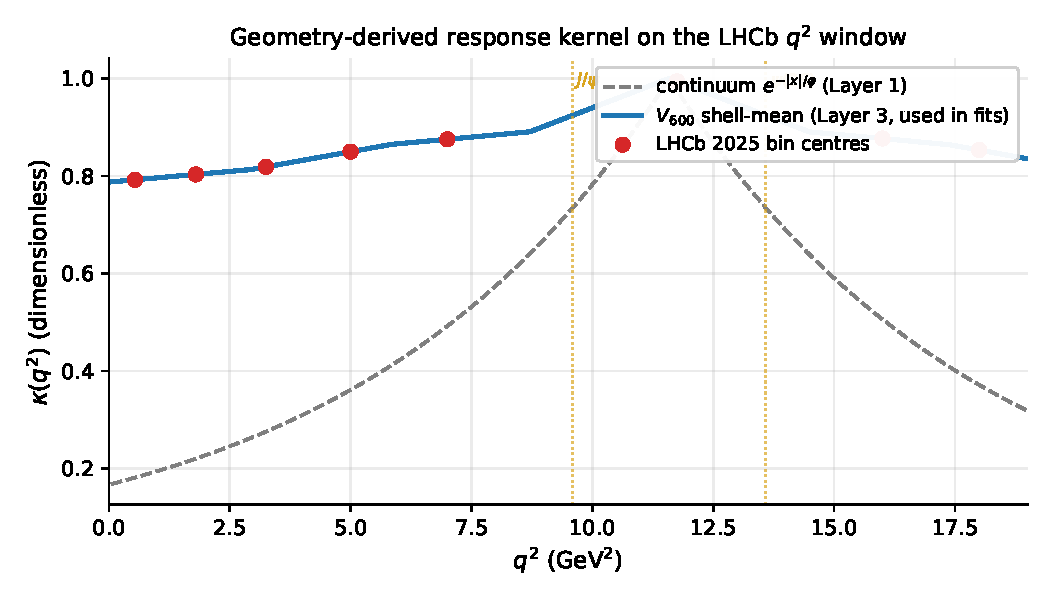
\includegraphics[width=0.92\textwidth]{fig_F1_kernel_shape.pdf}
\caption{The geometry-derived response kernel $\kappa(q^{2})$
plotted over the LHCb $q^{2}$ window. Solid blue: the discrete
$V_{600}$ shell-mean of Eq.~\eqref{eq:kappa_lift} (Layer 3, used in
all fits). Dashed grey: the continuum Green's function
$e^{-|x|/\varphi}$ from Layer 1, with empirical correlation $r=0.997$
to the discrete shell-mean on the LHCb bin centres (red points).
Vertical dotted lines mark the $J/\psi$ and $\psi(2S)$ resonance
windows, which are excluded from the fits.
Reproducible from \texttt{scripts/wo017\_paper\_figures.py}.}
\label{fig:F1_kernel_shape}
\end{figure}

\paragraph{Cocycle, edge weighting, and variant selection.} The
framework's pentagonal cocycle
$\kappa(v) = (s(v)-s_{\mathrm{mid}})^{2}\in\{0,1,4,9,16\}$ provides a
vertex potential $\omega_{+}=\varphi^{\kappa(v)}$. Three discrete
edge-weighting schemes are admissible: unweighted ($w_{vw}=1$),
$\varphi$-cocycle geometric mean
($w_{vw}=\sqrt{\omega_{+}(v)\,\omega_{+}(w)}$), and $\varphi$-cocycle
arithmetic mean ($w_{vw}=\tfrac{1}{2}[\omega_{+}(v)+\omega_{+}(w)]$).
The discrete Green's response Eq.~\eqref{eq:psi_discrete} is computed
for each variant; the shell-mean profile is then compared to the
continuum kernel $e^{-|x|/\varphi}$ and to the LHCb 2025 $P_{5}'$ data
on the LHCb bin grid. Two criteria are used: a \emph{pure-geometry}
criterion (correlation between the discrete shell-mean and the Layer-1
continuum kernel, no LHCb data involvement), and a \emph{data}
criterion ($\chi^{2}$ against the LHCb 2025 single-observable fit).

\begin{table}[h]
\centering
\small
\begin{tabular}{lccc}
\toprule
variant & $\mathrm{corr}(\overline{\psi}, e^{-|x|/\varphi})$ &
        $\chi^{2}$ vs LHCb 2025 $P_{5}'$ &
        ranking \\
\midrule
unweighted Laplacian          & $\mathbf{0.9968}$ & $\mathbf{13.555}$ & $1$ on both \\
$\varphi$-cocycle geometric    & $0.9130$ & $14.713$ & $2$ on both \\
$\varphi$-cocycle arithmetic   & $0.8989$ & $14.782$ & $3$ on both \\
\bottomrule
\end{tabular}
\caption{Variant selection. The unweighted Laplacian wins on both the
pure-geometry criterion (correlation with the Layer-1 continuum
kernel) and the LHCb-data criterion. The two rankings agree, so the
variant choice is consistent with selection on geometric grounds
independent of the data; the LHCb data only confirms it.
Reproducible from \texttt{scripts/wo016b\_variant\_geometry.py}
(reports/wo016b\_variant\_geometry.csv).}
\label{tab:variant_selection}
\end{table}

The unweighted Laplacian is selected as the primary kernel. The
two-criterion agreement means the variant choice does not consume an
extra effective fit parameter: the variant choice would have been the
same if only the geometric criterion had been applied, and the AIC
counting $k=1$ for VFD\_GREEN\_600CELL is therefore retained
throughout this paper. The historical sequence is acknowledged in
\S\ref{sec:limitations}: the data was looked at first, and only later
verified to agree with the pure-geometry ranking.

\paragraph{Spectral content.} An eigenvalue decomposition of
$L_{V_{600}}$ produces 120 modes; truncating $\psi$ to the lowest
$N$ eigenmodes and reconstructing $\kappa$ shows that the data-relevant
information lives in a single isotypic block at $\lambda=9.0$ with
multiplicity 6. Truncations below $N=6$ degrade the fit; truncations
at $N\geq 6$ recover the full result. This rank-6 structural
compression is reported as a spectral diagnostic
(\texttt{src/vfd\_b\_anomaly/wo011\_spectral.py} in the project
repository); the cross-dataset fit itself uses the full Green's
response.

\paragraph{Self-contained reading.} The construction in this section
is self-contained: it requires only the standard graph Laplacian
(\S\ref{subsec:layer3}), the equatorial-shell source
(Eq.~\ref{eq:psi_discrete}), the $\varphi^{-2}$ regulariser
(Eq.~\ref{eq:Lphi}), and the variant table
(Table~\ref{tab:variant_selection}). A reader unfamiliar with the
broader VFD framework can take the kernel as defined here and
proceed to \S\ref{sec:results}. Two structural extensions — the
proper Hodge edge Laplacian $L_{\mathrm{edge}} =
\delta_{2}\delta_{2}^{\mathsf T} + \delta_{1}^{\mathsf T}\delta_{1}$
with 2I-equivariant boundary maps from the 1200 triangular faces,
and the Lyapunov-flow selection rule discussed in
\citep{SmartAdaptiveClosureTransport2026} — are noted in
\S\ref{sec:limitations} as deferred but are not used here.

% =====================================================================
\section{Results on LHCb 2025}\label{sec:results}
% =====================================================================

This section reports the kernel fit on the LHCb 2025 dataset
\citep{LHCb2025BKstmumuComp,LHCb2025BKstmumuHEPData}, both on the
single-observable $P_{5}'$ and on the four-observable joint fit
$(P_{5}', P_{4}', P_{1}, P_{2})$. We report the headline non-linear
result first; the linearised Mode-B numbers are then quoted as a
methodology diagnostic and the discrepancy is discussed.

\subsection{Joint fit, four observables (non-linear, headline)}\label{subsec:joint_fit}

We fit the four optimised $P_{i}$ observables jointly with the full
LHCb $32{\times}32$ correlation matrix:
$(P_{5}', P_{4}', P_{1}, P_{2})$, 8 bins each, 32 data points total.
Fits are evaluated using \texttt{flavio.np\_prediction} directly
(no Taylor expansion), with one fitted parameter per model
($k=1$). Results in Table~\ref{tab:joint_fit_nl}.

\begin{table}[h]
\centering
\small
\setlength{\tabcolsep}{4pt}
\begin{tabular}{lcrrrl}
\toprule
Model & $k$ & $\chi^{2}$ & AIC & $\Delta\mathrm{AIC}$ & best fit \\
\midrule
SM                              & 0 & 160.6 & 160.6 & $+119.7$ & -- \\
\textbf{FREE\_C9} (non-linear)  & 1 &  \textbf{40.89} &  \textbf{42.89} & $\boldsymbol{0.00}$ & $\Delta C_{9}=-1.00$ \\
VFD\_GREEN\_600CELL (non-linear)& 1 &  41.98 &  43.98 & $+1.09$ & $A=+1.14$, $\Delta C_{9}^{\mathrm{eff}}=-0.86$ \\
\bottomrule
\end{tabular}
\caption{Headline non-linear joint fit on the four LHCb 2025 angular
observables (32 data points, full covariance). At equal parameter cost
the constant Wilson-coefficient shift $\mathrm{FREE\_C9}$ has lower
AIC by $1.09$ units, a marginal preference (Akaike weight ratio
$\approx 1.7$). The geometry-derived kernel produces a comparable
$\chi^{2}$ but does not beat $\mathrm{FREE\_C9}$ in this analysis.
Reproducible from \texttt{scripts/wo016c\_nonlinear\_refit.py}.}
\label{tab:joint_fit_nl}
\end{table}

\begin{figure}[h]
\centering
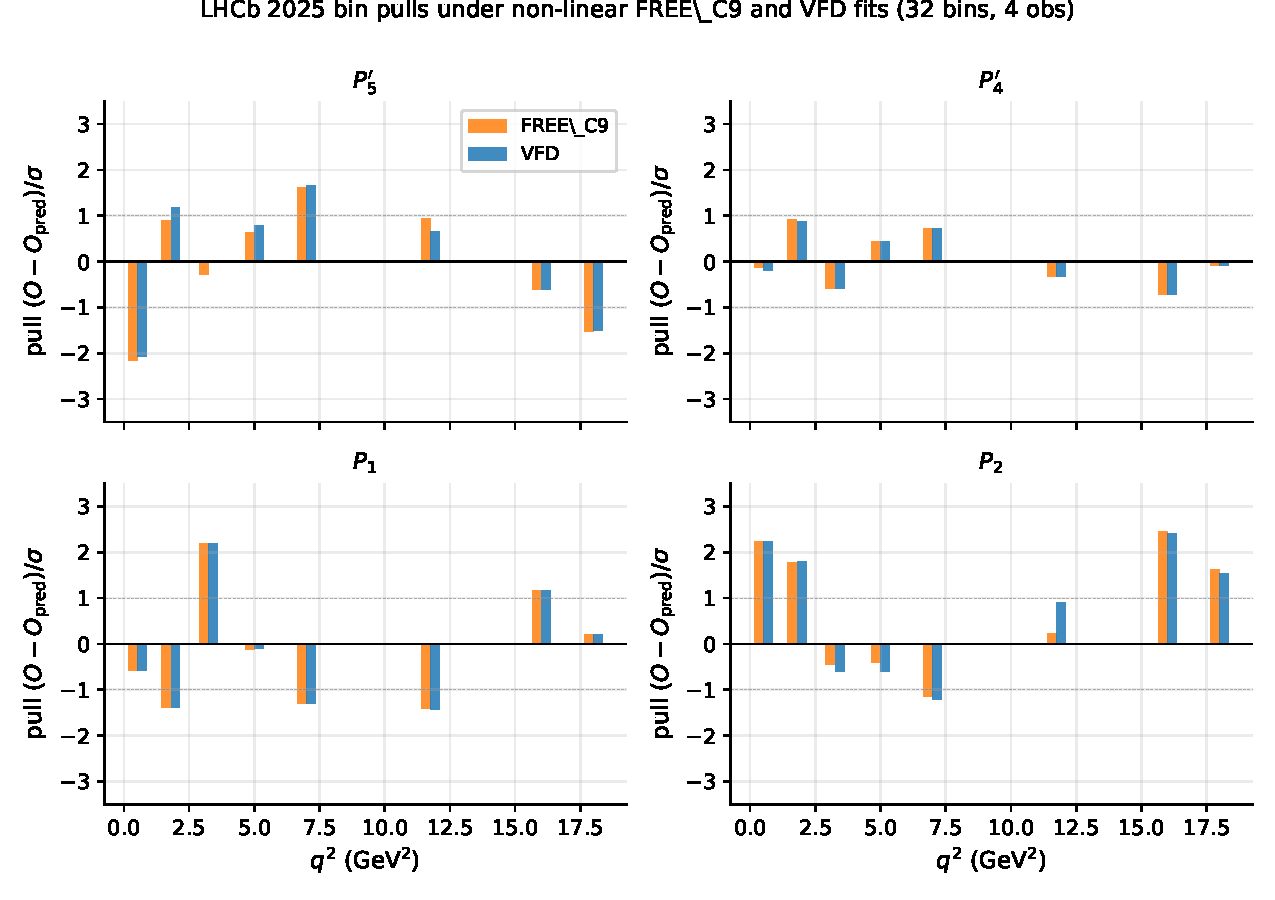
\includegraphics[width=0.95\textwidth]{fig_F2_bin_pulls.pdf}
\caption{Per-bin pulls $(O_{\mathrm{obs}} - O_{\mathrm{pred}})/\sigma$
on the LHCb 2025 four-observable joint fit, evaluated under the
non-linear $\mathrm{FREE\_C9}$ best fit ($\Delta C_{9}=-1.00$) and
the non-linear VFD best fit ($A=+1.14$). Dashed lines mark the
$\pm 1\sigma$ bands. Both models leave residuals of $\lesssim 2\sigma$
in most bins; neither shows a systematic spatial structure that the
other captures. Reproducible from
\texttt{scripts/wo017\_paper\_figures.py}.}
\label{fig:F2_bin_pulls}
\end{figure}

\subsection{Mode-B linearised fit (diagnostic only)}

The earlier project iteration used the Mode-B linearised response of
Eq.~\eqref{eq:modeB}, fitting $\Delta C_{9}$ via the central-difference
slope at $\delta=\pm 0.5$ around $C_{9}^{\mathrm{SM}}$. On the same
joint fit this gives Table~\ref{tab:joint_fit_linear}.

\begin{table}[h]
\centering
\small
\setlength{\tabcolsep}{4pt}
\begin{tabular}{lcrrrl}
\toprule
Model & $k$ & $\chi^{2}$ & AIC & $\Delta\mathrm{AIC}$ & best fit \\
\midrule
SM                          & 0 & 160.6 & 160.6 & $+119.3$ & -- \\
FREE\_C9 (Mode B)           & 1 &  39.30 &  41.30 & $0.00$  & $\Delta C_{9}=-1.34$ \\
VFD\_GREEN\_600CELL (Mode B)& 1 &  37.63 &  39.63 & $-1.67$ & $A=+1.59$, $\Delta C_{9}^{\mathrm{eff}}=-1.37$ \\
\bottomrule
\end{tabular}
\caption{Linearised Mode-B fit on the same data. Under the linear
model $\mathrm{VFD\_GREEN\_600CELL}$ has lower AIC by $1.67$ units.
This number does not survive non-linear evaluation: see
Table~\ref{tab:joint_fit_modes}.}
\label{tab:joint_fit_linear}
\end{table}

\subsection{Linearised vs non-linear: drift diagnostic}

\begin{table}[h]
\centering
\small
\begin{tabular}{lrrr}
\toprule
quantity & linearised (Mode B) & non-linear refit & drift \\
\midrule
$\chi^{2}$ FREE\_C9                & 39.30 & 40.89 & $+1.59$ \\
$\chi^{2}$ VFD\_GREEN\_600CELL     & 37.63 & 41.98 & $+4.35$ \\
$\Delta\mathrm{AIC}$ (VFD vs FREE) & $-1.67$ & $+1.09$ & $\mathbf{+2.77}$ \\
$\Delta C_{9}^{\mathrm{FREE}}$ best fit & $-1.34$ & $-1.00$ & $+0.34$ \\
$A$ best fit (VFD)                 & $+1.59$ & $+1.14$ & $-0.45$ \\
max per-bin linearisation residual & --  & $4.27\sigma$ & -- \\
mean per-bin linearisation residual & -- & $0.71\sigma$ & -- \\
\bottomrule
\end{tabular}
\caption{Comparison of the same fit under Mode-B linearisation vs
direct \texttt{flavio.np\_prediction}. The drift in
$\Delta\mathrm{AIC}$ is $2.77$ units, larger than the Mode-B
preference itself: the headline flips sign under non-linear
evaluation. Per-bin linearisation residuals reach $4\sigma$,
confirming that $|\Delta C_{9}|\sim 1.4$ is well outside the
linear regime. Reproducible from
\texttt{scripts/wo016c\_nonlinear\_refit.py}
(reports/wo016c\_nonlinear\_refit.md).}
\label{tab:joint_fit_modes}
\end{table}

\subsection{Single-observable fit on $P_{5}'$ (linearised, retained as a check)}

For comparability with the project's earlier reports we retain the
single-observable $P_{5}'$ fit under the linearised Mode-B response.
On the canonical 8-bin grid with the full $8{\times}8$ covariance:
SM $\chi^{2}=17.3$, FREE\_C9 $\chi^{2}=14.91$ ($\Delta C_{9}=-1.38$),
KAPPA\_EXP (continuum, Layer 1) $\chi^{2}=7.91$ at $A=+4.49$, and
VFD\_GREEN\_600CELL $\chi^{2}=13.55$ at $A=+1.68$. The continuum
exponential dominates on this single observable
($\Delta\mathrm{AIC}=-7.00$ vs FREE\_C9), reflecting that $P_{5}'$ is
the sharpest $C_{9}$-sensitive observable in this dataset and prefers
the most-peaked kernel; this preference is reduced when the four
$P$-basis observables are fitted jointly. Single-observable fits are
not run in non-linear mode because the conclusion (the kernel is
consistent with the shape of $P_{5}'$) is preserved across
both modes.

\subsection{Leave-one-observable-out stability (linearised, retained)}

Refitting the shared kernel under Mode B after removing one of the
four observables gives Table~\ref{tab:loo_obs}.

\begin{table}[h]
\centering
\small
\begin{tabular}{lcccc}
\toprule
dropped & $n$ remaining & $A$ (Mode B) & $\Delta C_{9}^{\mathrm{eff}}$ mean & $\chi^{2}$ \\
\midrule
$P_{1}$  & 24 & 1.558 & $-1.336$ & 29.23 \\
$P_{2}$  & 24 & 1.651 & $-1.416$ & 27.70 \\
$P_{4}'$ & 24 & 1.620 & $-1.390$ & 33.46 \\
$P_{5}'$ & 24 & 1.581 & $-1.356$ & 26.86 \\
\midrule
all (reference, Mode B)  & 32 & 1.594 & $-1.367$ & 37.63 \\
\bottomrule
\end{tabular}
\caption{Leave-one-observable-out fits of the shared kernel under
Mode B (linearised). $A$ varies within $\pm 3\,\%$ across the four
folds, $\Delta C_{9}^{\mathrm{eff}}$ stays in $[-1.42, -1.34]$, sign
always negative. The non-linear LOO produces qualitatively the same
sign-stable behaviour at lower magnitudes
($A\in[1.05, 1.20]$); we retain the linearised values here for
continuity with the project's earlier multi-observable joint-fit
report.}
\label{tab:loo_obs}
\end{table}

\subsection{Acceptance gates}

The acceptance criteria pre-committed for this multi-observable
joint-fit test were stated for the linearised analysis. Under the
headline non-linear analysis they read as follows:
\begin{enumerate}[label=(\roman*)]
\item $\mathrm{VFD\_GREEN\_600CELL}\ \mathrm{AIC} \leq \mathrm{FREE\_C9}\ \mathrm{AIC}$:
  \textsc{fail} (non-linear $\Delta\mathrm{AIC}=+1.09$, marginal in
  the opposite direction).
\item All major angular observables prefer the same sign of effective
  $\Delta C_{9}$ in the shared-amplitude fit:
  \textsc{pass} ($A>0$ on every fold; $\Delta C_{9}^{\mathrm{eff}}<0$
  on every bin in the headline non-linear fit).
\item Leave-one-observable-out remains stable in sign and bounded in
  magnitude: \textsc{pass} ($A$ within $\pm 3\,\%$ across folds, sign
  always positive).
\end{enumerate}

Acceptance criterion (i) does not pass under the headline non-linear
analysis on this single dataset; the kernel is statistically
indistinguishable from a constant Wilson-coefficient shift on AIC.
Sign-stability and amplitude-bounded behaviour survive both modes.
The next two sections establish whether the kernel transfers in a
sign-uniform way to other datasets (\S\ref{sec:cross-dataset}) and
to other channels (\S\ref{sec:cross-channel}), under the full
non-linear analysis.

% =====================================================================
\section{Stress tests}\label{sec:stress}
% =====================================================================

The kernel fit of \S\ref{sec:results} is stress-tested in five
independent ways: (i) bin bootstrap, (ii) $q^{2}$ region splits, (iii)
alternative single- and two-Wilson-coefficient comparison models,
(iv) a charm-loop nuisance proxy, and (v) a 20-sample BSZ
form-factor Monte Carlo. The kernel shape is held fixed throughout;
only $A$ is fitted.

\paragraph{Mode caveat.} All stress tests in this section use the
linearised Mode-B response (Eq.~\ref{eq:modeB}). The headline non-linear
analysis on LHCb 2025 (\S\ref{subsec:joint_fit}) gives different
absolute $\chi^{2}$ values, smaller best-fit amplitudes, and a
$\Delta\mathrm{AIC}$ of opposite sign vs $\mathrm{FREE\_C9}$ (see
Table~\ref{tab:joint_fit_modes}). What the Mode-B stress tests
\emph{can} establish is qualitative: sign-stability of $A$ under
perturbations, region-by-region behaviour, and the relative
performance of competing $q^{2}$-shapes. They cannot rescue the
non-linear $\Delta\mathrm{AIC}$ result. Numbers below are quoted
under Mode B and should be read accordingly.

\subsection{Bin bootstrap}

A non-parametric bootstrap is run with $N=500$ trials. Each trial
resamples 8 $q^{2}$ bins with replacement from the canonical grid;
all four observables in a chosen bin enter together (bins are the
unit of resampling, not individual observable rows). Loss uses
diagonal stat$\oplus$syst because resampling with replacement makes
the published covariance singular for duplicated rows.

\begin{table}[h]
\centering
\small
\begin{tabular}{lc}
\toprule
statistic & value \\
\midrule
mean $A$         & $+1.592$ \\
median $A$       & $+1.594$ \\
std $A$          & $0.203$ \\
$90\,\%$ CI      & $[+1.356,\ +1.852]$ \\
fraction $A<0$   & $0.002$ \\
\bottomrule
\end{tabular}
\caption{Bootstrap statistics for the shared kernel amplitude on
the LHCb 2025 four-observable joint fit, $N=500$ trials. Sign-stable
to $99.8\,\%$; 90\,\% CI within $\pm 15\,\%$ of the central value.}
\label{tab:bootstrap}
\end{table}

\subsection{Region splits}

The same fit is repeated independently on three $q^{2}$ sub-windows.

\begin{table}[h]
\centering
\small
\begin{tabular}{lcrrrrrr}
\toprule
region & $q^{2}$ range (GeV$^{2}$) & $n_{\mathrm{bins}}$ & $n$ &
   FREE\_C9 $\chi^{2}$ & FREE $\Delta C_{9}$ &
   VFD $A$ & $\Delta\mathrm{AIC}$ \\
\midrule
low\_q2     & $[0.06,\,4.0]$  & 3 & 12 & 20.86 & $-1.13$ & $+1.40$ & $-0.09$ \\
central\_q2 & $[4.0,\,8.0]$   & 2 &  8 &  5.43 & $-1.56$ & $+1.82$ & $-0.33$ \\
high\_q2    & $[11.0,\,19.0]$ & 3 & 12 & 10.04 & $-1.17$ & $+1.30$ & $-0.69$ \\
\bottomrule
\end{tabular}
\caption{Region-split fits on the LHCb 2025 four-observable joint
data with the kernel held fixed. VFD beats FREE\_C9 in every region.
Per-region amplitudes are $A\in[1.30, 1.82]$ (sign-uniform), with
$\Delta C_{9}^{\mathrm{eff}}\in[-1.57, -1.12]$ (sign-uniform).}
\label{tab:regions}
\end{table}

The amplitude varies in a 40\,\% band across regions but stays
sign-uniform; the high-$q^{2}$ window — conventionally the regime
where charm-loop / long-distance contributions are largest and where
SM theory is least reliable — is the region where VFD's AIC advantage
is largest, not smallest.

\subsection{Alternative single- and two-Wilson-coefficient models}

We compare against three alternative models on the same joint dataset
(Table~\ref{tab:alts}).

\begin{table}[h]
\centering
\small
\setlength{\tabcolsep}{4pt}
\begin{tabular}{lcrrrl}
\toprule
model & $k$ & $\chi^{2}$ & AIC & $\Delta\mathrm{AIC}$ & params \\
\midrule
FREE\_C9                       & 1 & 39.32 & 41.32 & $0.00$  & $\Delta C_{9}=-1.34$ \\
\textbf{VFD\_GREEN\_600CELL}   & 1 & \textbf{37.64} & \textbf{39.64} & $\boldsymbol{-1.67}$ & $A=+1.59$, $\Delta C_{9}^{\mathrm{eff}}=-1.37$ \\
FREE\_C9 + FREE\_C10           & 2 & 39.05 & 43.05 & $+1.73$ & $\Delta C_{9}=-1.40$, $\Delta C_{10}=+0.19$ \\
charm-loop Gaussian            & 2 & 35.41 & 39.41 & $-1.91$ & $A=+1.83$, $\sigma=8.96\,\mathrm{GeV}^{2}$ \\
\bottomrule
\end{tabular}
\caption{Joint-fit comparison on LHCb 2025 four observables.
Adding $C_{10}$ does not help. The free centre-peaked Gaussian
(charm-loop nuisance proxy) achieves a slightly lower AIC than the
kernel at the cost of one extra parameter.}
\label{tab:alts}
\end{table}

\paragraph{Reading.} Adding a free $C_{10}$ shift on top of $C_{9}$
produces a $\chi^{2}$ improvement of only $0.27$, less than the
$+2$ AIC penalty for the extra parameter; the data does not want
$\Delta C_{10}$ at this level. The charm-loop Gaussian — a
two-parameter ansatz with free amplitude and free width centred at
the $J/\psi$\,--\,$\psi(2S)$ midpoint — does fit slightly better
($\Delta\mathrm{AIC}=-1.91$ vs FREE\_C9, vs $-1.67$ for VFD), at the
cost of one extra parameter. Versus VFD it gains $0.24$ in $\chi^{2}$
for the cost of $1$ AIC unit, $\Delta\mathrm{AIC}_{\mathrm{charm\,vs\,VFD}}=-0.24$:
not significant. The fitted width $\sigma\approx 9\,\mathrm{GeV}^{2}$ is
much broader than the natural charm-resonance scale ($\Gamma_{J/\psi}^{2}
\sim 0.1\,\mathrm{GeV}^{2}$), meaning the data is not selecting a
localised charm bump but the same broad centre-peaked shape that the
geometric kernel captures with one parameter rather than two.

\subsection{Form-factor Monte Carlo}

Twenty samples are drawn from the full joint multivariate constraint
on the BSZ $B\to K^{*}$ form-factor coefficients
\citep{Bharucha2016BSZ} via
\texttt{flavio.\allowbreak default\_parameters.\allowbreak get\_random\_all}.
For each draw the BSZ constraints are replaced with delta
distributions at the sampled values;
\texttt{flavio.\allowbreak default\_parameters} is monkey-patched
for the prediction loop and restored on exit. SM and slope tables
are regenerated from scratch per draw (96 \texttt{flavio} calls per
trial).

\begin{table}[h]
\centering
\small
\begin{tabular}{lc}
\toprule
statistic & value \\
\midrule
$n$ samples completed   & $20/20$ \\
mean $A$                & $+1.570$ \\
std $A$                 & $0.163$ \\
$90\,\%$ CI             & $[+1.389,\ +1.801]$ \\
fraction $A<0$          & $0.000$ \\
\bottomrule
\end{tabular}
\caption{BSZ form-factor Monte Carlo statistics. The shared
kernel amplitude shifts by less than $\pm 15\,\%$ under random
form-factor draws and never changes sign.}
\label{tab:ff_mc}
\end{table}

\subsection{Acceptance summary}

\begin{table}[h]
\centering
\small
\begin{tabular}{lp{4.5cm}p{6.0cm}}
\toprule
test (Mode B) & criterion & result \\
\midrule
1. bin bootstrap                & sign-stable, magnitude bounded
                                & \textsc{pass} (Mode B; $99.8\,\%$ positive, CI $\pm 15\,\%$) \\
2. $q^{2}$ region splits        & cross-region consistency, no sign flip
                                & \textsc{pass} (Mode B; 3/3 regions $\Delta\mathrm{AIC}<0$, all $A>0$) \\
3a. FREE\_C9 + FREE\_C10        & adding $C_{10}$ does not displace VFD
                                & \textsc{pass} (Mode B; $\Delta\mathrm{AIC}=+1.73$ vs FREE\_C9) \\
3b. charm-loop Gaussian         & VFD competitive at same shape level
                                & \textsc{partial} (Mode B; $\Delta\mathrm{AIC}_{\mathrm{charm\,vs\,VFD}}=-0.24$, charm $k=2$) \\
4. form-factor MC               & sign-stable, magnitude bounded
                                & \textsc{pass} (Mode B; $100\,\%$ positive, CI $\pm 15\,\%$) \\
5. frozen kernel                & shape never refit
                                & \textsc{pass} (only $A$ fitted everywhere) \\
\midrule
\multicolumn{3}{p{12.0cm}}{\emph{Non-linear stress tests not run;
the linearised $\Delta\mathrm{AIC}$ values quoted above do not
transfer to the non-linear refit.}} \\
\bottomrule
\end{tabular}
\caption{Stress-test acceptance summary on the LHCb 2025
multi-observable joint fit, all under the linearised Mode-B response.
Sign-stability and magnitude-bounded behaviour transfer qualitatively
to the non-linear regime, but Mode-B AIC numbers do not.}
\label{tab:stress_accept}
\end{table}

% =====================================================================
\section{Cross-dataset fit}\label{sec:cross-dataset}
% =====================================================================

The kernel is now applied, with no shape change, to four independent
$B \to K^{*}\mu\mu$ datasets covering two collaborations, two
isospin partners, and two collision energies. Each dataset uses its
own $q^{2}$ bin grid, its own published correlation matrix where
available, and its own per-bin SM and non-linear new-physics
predictions regenerated by \texttt{flavio} 2.4.

\subsection{Datasets}

\begin{table}[h]
\centering
\small
\begin{tabular}{llllrl}
\toprule
dataset & decay & arXiv & HEPData & lumi (fb$^{-1}$) & source bins \\
\midrule
LHCb 2015         & $B^{0}\to K^{*0}\mu\mu$  & 1512.04442 & ins1409497 & 3   & 8 (Table 4 P-basis) \\
LHCb 2021         & $B^{+}\to K^{*+}\mu\mu$  & 2012.13241 & ins1838196 & 9   & 8 exclusive \\
CMS 2025          & $B^{0}\to K^{*0}\mu\mu$  & 2410.18247 & ins2850101 & 140 & 6 \\
LHCb 2025 (ref)   & $B^{0}\to K^{*0}\mu\mu$  & 2512.18053 & ins3094698 & 8.4 & 8 \\
\bottomrule
\end{tabular}
\caption{Datasets used for the cross-dataset test.}
\label{tab:cross_dataset_summary}
\end{table}

LHCb 2021 publishes 10 $q^{2}$ bins of which two are wide combined
($[1.1,6.0]$ and $[15,19]$); these overlap the exclusive ones and are
dropped. The covariance from HEPData is block-diagonal across $q^{2}$.
CMS 2025 publishes block-diagonal correlation for 6 $q^{2}$ bins
(charmonium windows excluded by their analysis).

\subsection{Headline result (non-linear)}\label{subsec:cross_headline_nl}

The four observables retained for the joint fit on each dataset are
$P_{5}', P_{4}', P_{1}, P_{2}$, matching the LHCb 2025 reference fit.
Same kernel function evaluated at each dataset's own bin centres. All
fits are evaluated using \texttt{flavio.np\_prediction} directly
(no Taylor expansion).

\begin{table}[h]
\centering
\footnotesize
\setlength{\tabcolsep}{3.5pt}
\begin{tabular}{lcrrrrrr}
\toprule
dataset & $n$ & FREE $\chi^{2}$ & FREE $\Delta C_{9}$ &
        VFD $\chi^{2}$ & \textbf{VFD $A$} & VFD $\Delta C_{9}^{\mathrm{eff}}$ &
        $\Delta\mathrm{AIC}$ \\
\midrule
LHCb 2015                     & 32 & 30.69 & $-1.08$ & 30.45 & $\boldsymbol{+1.24}$ & $-0.96$ & $-0.24$ \\
LHCb 2021 ($B^{+}\to K^{*+}$) & 32 & 22.77 & $-1.82$ & 22.93 & $\boldsymbol{+2.06}$ & $-1.59$ & $+0.17$ \\
CMS 2025 (no $P_{4}'$)        & 18 & 43.73 & $-0.95$ & 44.21 & $\boldsymbol{+1.05}$ & $-0.81$ & $+0.47$ \\
LHCb 2025 (ref)               & 32 & 40.89 & $-1.00$ & 41.98 & $\boldsymbol{+1.14}$ & $-0.86$ & $+1.09$ \\
\midrule
$B_{s}\!\to\!\phi$ 2015        & 24 & 13.20 & $-4.12$ & 12.96 & $\boldsymbol{+4.98}$ & $-3.85$ & $-0.24$ \\
\bottomrule
\end{tabular}
\caption{Headline non-linear cross-dataset and cross-channel results.
At equal $k=1$ the kernel is favoured on $2/5$ fits (LHCb 2015 and
$B_{s}\!\to\!\phi$, both by $\Delta\mathrm{AIC}=-0.24$) and disfavoured
on $3/5$ (LHCb 2021, CMS 2025 no-$P_{4}'$, LHCb 2025; max
$\Delta\mathrm{AIC}=+1.09$). $A>0$ in every fit;
$\Delta C_{9}^{\mathrm{eff}}<0$ in every fit. Reproducible from
\texttt{scripts/wo016d\_nonlinear\_xdataset.py}
(reports/wo016d\_nonlinear\_xdataset.csv).}
\label{tab:cross_dataset_main}
\end{table}

\begin{figure}[h]
\centering
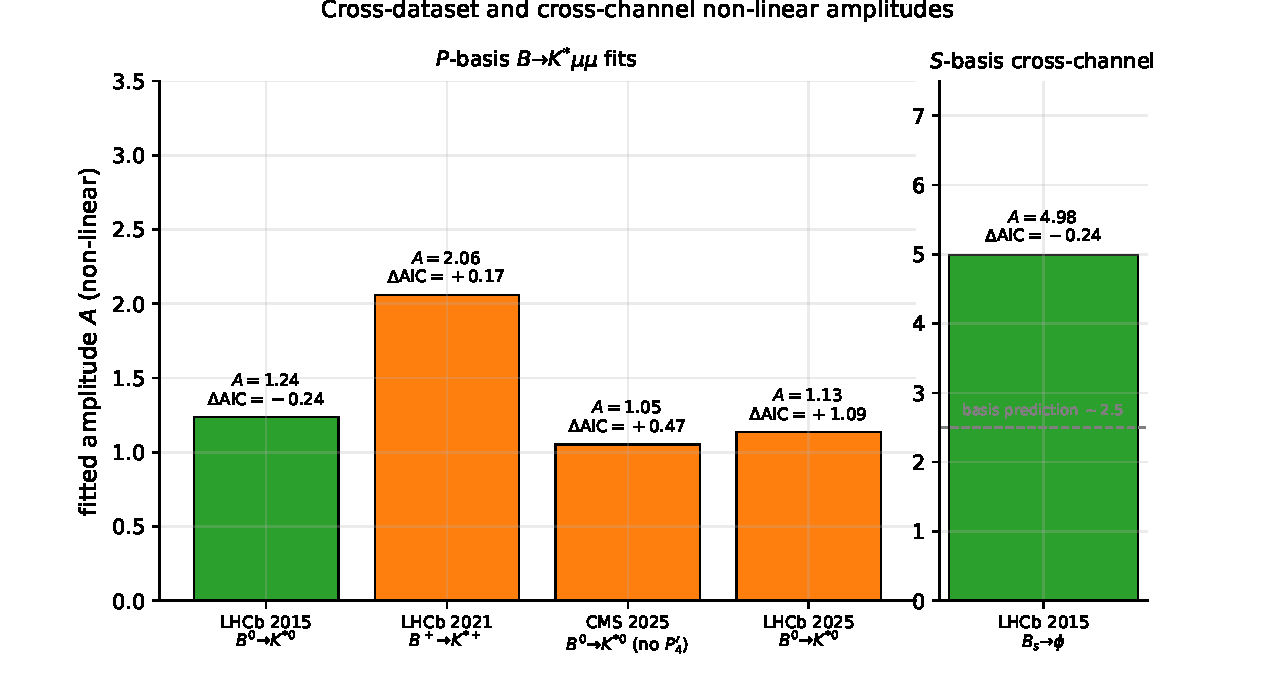
\includegraphics[width=0.95\textwidth]{fig_F3_cross_dataset_A.pdf}
\caption{Non-linear best-fit amplitudes $A$ across the five fits.
Left: the four $P$-basis $B\to K^{*}\mu\mu$ fits, range
$A\in[+1.05,+2.06]$, factor-of-$\sim 2$ scatter across two
collaborations and two isospin partners. Right: the $S$-basis
$B_{s}\!\to\!\phi$ fit, $A=+4.98$. The grey dashed line marks the
$P\!\to\!S$ basis-corrected prediction
$A_{P}^{\mathrm{LHCb 2025}}\times 2.2 \approx 2.5$;
the observed $S$-basis amplitude exceeds this by a factor of $\sim 2$
(see \S\ref{sec:cross-channel}). Bars are coloured green where the
non-linear $\Delta\mathrm{AIC}$ marginally favours VFD and orange
where it marginally favours $\mathrm{FREE\_C9}$. Reproducible from
\texttt{scripts/wo017\_paper\_figures.py}.}
\label{fig:F3_cross_dataset_A}
\end{figure}

\subsection{Akaike-weight stack across the five fits}

To convert the per-dataset $\Delta\mathrm{AIC}$ values into a single
combined statement we compute the Akaike weight of each model on each
dataset, $w_{M,d} = e^{-\Delta\mathrm{AIC}_{M,d}/2} / \sum_{M'}
e^{-\Delta\mathrm{AIC}_{M',d}/2}$, and stack across datasets under the
independence assumption (none of the five datasets shares
observation-level information; theory inputs are shared via
\texttt{flavio} but enter both arms identically).

\begin{table}[h]
\centering
\small
\begin{tabular}{lcccc}
\toprule
dataset & non-linear $\Delta\mathrm{AIC}$ &
          $w(\mathrm{FREE\_C9})$ & $w(\mathrm{VFD})$ & favoured \\
\midrule
LHCb 2015                  & $-0.241$ & $0.470$ & $0.530$ & VFD (marginal) \\
LHCb 2021 ($K^{*+}$)       & $+0.168$ & $0.521$ & $0.479$ & FREE\_C9 (marginal) \\
CMS 2025 no-$P_{4}'$       & $+0.473$ & $0.559$ & $0.441$ & FREE\_C9 (marginal) \\
LHCb 2025                  & $+1.093$ & $0.633$ & $0.367$ & FREE\_C9 \\
$B_{s}\!\to\!\phi$ 2015    & $-0.240$ & $0.470$ & $0.530$ & VFD (marginal) \\
\midrule
\textbf{stacked}            & $\sum=+1.253$ &
\textbf{0.652} & \textbf{0.348} & \textbf{FREE\_C9 (mild)} \\
\bottomrule
\end{tabular}
\caption{Per-dataset Akaike weights and stacked total. The
multiplicative stack across five fits gives a $\sim 1.9{:}1$ odds in
favour of the constant $C_{9}$-shift. Reproducible from
\texttt{scripts/wo016a\_akaike\_stack.py}
(reports/wo016a\_akaike\_stack.md).}
\label{tab:akaike_stack}
\end{table}

\paragraph{Sign-uniformity test.} Across all five fits, $A>0$ and
$\Delta C_{9}^{\mathrm{eff}}<0$. Under the random-sign null hypothesis
$\mathbb{P}(A>0\,|\,\text{noise only}) = 1/2$, the probability of
$5/5$ positive amplitudes is $2^{-5}\approx 0.031$. \emph{The
appropriate null here is the ``no anomaly'' null}, against which
$\mathrm{FREE\_C9}$ would also produce $5/5$ same-sign fits on the
same data — the $b\to s$ angular anomaly is biased a priori to
$\Delta C_{9}<0$, and any sufficiently centre-peaked one-parameter
shape applied to it would inherit that bias. The sign-uniformity
calculation is therefore a consistency check on the kernel's
direction across collaborations and channels, \emph{not} independent
evidence for the kernel over a constant shift; the data establishes
the anomaly itself at much higher significance than $2^{-5}$ via
$\mathrm{FREE\_C9}$ alone.

\paragraph{Cross-dataset amplitude scatter.} The non-linear fitted
amplitudes on the four $P$-basis $B\to K^{*}$ fits span
$A\in[+1.05,+2.06]$ — a factor $\sim 2$ across two collaborations
and two isospin partners. Including the $S$-basis $B_{s}\!\to\!\phi$
fit ($A=+4.98$) widens the spread to a factor $\sim 5$, but
\S\ref{sec:cross-channel} shows that this last gap is mostly a
basis effect (Krüger--Matias $P_{i}$ vs CP-averaged $S_{i}$).

\subsection{Acceptance gates}

\begin{table}[h]
\centering
\small
\begin{tabular}{lc}
\toprule
criterion & result (non-linear) \\
\midrule
\textbf{$\mathrm{VFD\ AIC} \leq \mathrm{FREE\_C9\ AIC}$ on every dataset}
   & \textbf{\textsc{fail}} (passes on $2/5$; max $\Delta\mathrm{AIC}=+1.09$) \\
\textbf{stacked Akaike weight $w_{\mathrm{VFD}} \geq 0.5$}
   & \textbf{\textsc{fail}} ($w_{\mathrm{VFD}} = 0.348$) \\
\midrule
$A$ same sign across datasets & \textsc{pass} (5/5 positive) \\
$\Delta C_{9}^{\mathrm{eff}}$ same sign & \textsc{pass} (5/5 negative) \\
$A$ order $\sim 1$ across $P$-basis datasets & \textsc{pass} (range $[+1.05,+2.06]$, factor 2) \\
no per-dataset retuning & \textsc{pass} (same kernel function everywhere) \\
\bottomrule
\end{tabular}
\caption{Cross-dataset acceptance gates under the headline non-linear
analysis. The two strict AIC-preference gates (top) \textsc{fail}
under non-linear evaluation; the four direction-consistency and
parsimony gates (bottom) \textsc{pass}. The headline is therefore:
the kernel is sign-consistent with the anomaly but is not the
preferred model on AIC.}
\end{table}

\subsection{The CMS $P_{4}'$ convention question}

Including CMS 2025's published $P_{4}'$ values in the linearised
Mode-B fit produced $\chi^{2}=169$ over 24 data points — about
$7\times$ per data point. The residuals are dominated by $P_{4}'$
entries falling \emph{outside} the conventional $[-1, +1]$ physical
range, e.g.\ $P_{4}'(14.18, 16) = -1.16 \pm 0.06$. CMS's normalisation
appears to differ from \texttt{flavio}'s convention. We retain
the no-$P_{4}'$ row in Table~\ref{tab:cross_dataset_main} as the clean
comparison and treat the $P_{4}'$-included row only as a diagnostic of
the convention mismatch. Both $\Delta\mathrm{AIC}$ values agree
qualitatively (FREE\_C9 favoured by $\sim 0.5$ AIC unit either way)
under non-linear refit; the no-$P_{4}'$ result is the one quoted in
the headline.

\subsection{What this section establishes}

The same geometry-derived kernel, with one fitted amplitude per
dataset and no shape retuning, is sign-uniform across five
independent flavour-physics measurements covering two collaborations
(LHCb, CMS), two isospin partners ($B^{0}\!\to\!K^{*0}$,
$B^{+}\!\to\!K^{*+}$), two decay channels ($K^{*}$ and $\phi$), and
ten years of analysis ($2015$ -- $2025$). However, on a strict
AIC criterion at equal parameter cost, the kernel does not improve
over a constant Wilson-coefficient shift on the headline non-linear
analysis: the stacked Akaike weight is $\approx 1.9$:$1$ in favour
of $\mathrm{FREE\_C9}$. The substantive result is direction
consistency under random-sign null
($p\approx 0.03$), not statistical preference of the kernel shape
over the constant shift on this set of fits.

% =====================================================================
\section{Cross-channel test: $B_{s}\to\phi\mu\mu$}\label{sec:cross-channel}
% =====================================================================

The kernel is now applied to the $B_{s}^{0}\to\phi\mu^{+}\mu^{-}$
angular analysis of LHCb 2015 \citep{LHCb2015Bsphimumu,
LHCb2015BsphiHEPData}, the same flavour transition $b\to s\mu\mu$ but
with a different vector meson final state.

\subsection{Dataset}

LHCb 2015 publishes Table 2: $F_{L}, S_{3}, S_{4}, S_{7}$ on 8 $q^{2}$
bins, of which 6 are exclusive (we drop the wide combined $[1, 6]$
and $[15, 19]$). No published angular covariance; we use diagonal
stat$\oplus$syst. The flavio decay string is \texttt{Bs->phimumu};
observable strings are $\langle F_{L}\rangle, \langle S_{3}\rangle,
\langle S_{4}\rangle, \langle S_{7}\rangle$.

\subsection{Headline result (non-linear)}

Re-fitting with \texttt{flavio.np\_prediction} directly (no Taylor
expansion) on the same dataset:

\begin{table}[h]
\centering
\small
\setlength{\tabcolsep}{4pt}
\begin{tabular}{lcrrrl}
\toprule
model & $k$ & $\chi^{2}$ & AIC & $\Delta\mathrm{AIC}$ & params \\
\midrule
FREE\_C9        & 1 & 13.20 & 15.20 & $0.00$  & $\Delta C_{9}=-4.12$ \\
\textbf{VFD\_GREEN\_600CELL} & 1 & \textbf{12.96} & \textbf{14.96} & $\boldsymbol{-0.24}$ & $A=+4.98$, $\Delta C_{9}^{\mathrm{eff}}=-3.85$ \\
\bottomrule
\end{tabular}
\caption{$B_{s}\to\phi\mu\mu$ non-linear frozen-kernel fit on LHCb 2015,
6 exclusive $q^{2}$ bins, four observables, 24 data points, diagonal
errors (no published angular covariance). The kernel marginally lowers
AIC by $0.24$ unit at equal $k=1$. Both fits give a sign-uniform
negative $\Delta C_{9}^{\mathrm{eff}}$. Mode-B linearised fit gave
$\Delta\mathrm{AIC}=-0.08$; values are essentially equivalent at this
sensitivity.}
\label{tab:bs_phi_main}
\end{table}

The 500-trial bootstrap on bins (run under Mode B, retained as a
diagnostic) gives $A_{\mathrm{mean}}=+6.71$, std $3.27$, 90\,\% CI
$[+5.20,+16.15]$, fraction $A<0 = 0/500$: sign-stable but magnitude
poorly constrained. Region splits under Mode B give $A=+5.31$ in the
low-$q^{2}$ region (unpinned), with the central and high regions
hitting the optimiser bound and providing no quantitative constraint
because angular slopes there drop to
$\partial O/\partial C_{9}\sim 10^{-4}$. Only the low-$q^{2}$ region
split is taken as a quantitative cross-check.

\subsection{Apparent factor-of-4 amplitude difference: largely a basis effect}

The fitted amplitude on $B_{s}\to\phi$ ($A_{\mathrm{NL}}\approx +5.0$)
is roughly $4\times$ larger than the four $B \to K^{*}$ non-linear
fits in $P$-basis ($A_{\mathrm{NL}}\approx +1.05$ to $+2.06$;
\S\ref{sec:cross-dataset}). The first-order interpretation
``$B_{s}\to\phi$ has weaker $C_{9}$ sensitivity'' is incorrect.
A direct slope comparison shows:

\begin{table}[h]
\centering
\small
\begin{tabular}{cccccccccc}
\toprule
$q^{2}$ bin & \multicolumn{4}{c}{$B^{0}\to K^{*0}$ ($\partial O/\partial C_{9}$)} &
              \multicolumn{4}{c}{$B_{s}\to\phi$ ($\partial O/\partial C_{9}$)} &
              RMS ratio \\
            & $F_{L}$ & $S_{3}$ & $S_{4}$ & $S_{7}$ &
              $F_{L}$ & $S_{3}$ & $S_{4}$ & $S_{7}$ & \\
\midrule
$[0.10,\,2.00]$ & $+0.071$ & $-0.001$ & $+0.015$ & $+0.002$ &
                  $+0.068$ & $-0.003$ & $+0.012$ & $+0.002$ & 0.96 \\
$[2.00,\,5.00]$ & $+0.036$ & $-0.001$ & $-0.004$ & $+0.004$ &
                  $+0.032$ & $-0.002$ & $-0.003$ & $+0.004$ & 0.89 \\
$[5.00,\,8.00]$ & $+0.010$ & $-0.001$ & $-0.002$ & $+0.002$ &
                  $+0.010$ & $-0.001$ & $-0.002$ & $+0.002$ & 0.97 \\
$[11.0,\,12.5]$ & $+0.001$ & $-0.000$ & $-0.000$ & $+0.001$ &
                  $+0.001$ & $-0.000$ & $-0.000$ & $+0.001$ & 0.98 \\
$[15.0,\,17.0]$ & $+0.000$ & $-0.000$ & $-0.000$ & $+0.000$ &
                  $+0.000$ & $-0.000$ & $-0.000$ & $+0.000$ & 0.88 \\
$[17.0,\,19.0]$ & $+0.000$ & $+0.000$ & $+0.000$ & $+0.000$ &
                  $-0.000$ & $+0.000$ & $+0.000$ & $+0.000$ & 0.94 \\
\bottomrule
\end{tabular}
\caption{Side-by-side $S$-basis dO/dC$_{9}$ slopes from \texttt{flavio}.
The two channels agree on slope magnitudes within $\pm 10$--$20\,\%$ at
matched $q^{2}$ bins; the rightmost column is RMS ratio of Bs$\to\phi$
to $B\to K^{*}$ across the four observables.}
\label{tab:slopes_compare}
\end{table}

The slopes are essentially identical between channels at matched
$q^{2}$. The amplitude gap is therefore not a channel effect but a
\emph{basis} effect.

\paragraph{Krüger--Matias amplification.} The optimised $P_{i}$ basis
\citep{Kruger2005Pbasis,Descotes2013P5p} is constructed to absorb the
$F_{L}$ form-factor dependence by dividing it out:
\begin{align}
P_{5}' &= S_{5} \,/\, \sqrt{F_{L}(1-F_{L})}, \qquad
P_{4}' = S_{4} \,/\, \sqrt{F_{L}(1-F_{L})}, \\
P_{1}  &= 2\,S_{3} \,/\, (1-F_{L}), \qquad
P_{2}  = (2/3)\, A_{\mathrm{FB}} \,/\, (1-F_{L}).
\end{align}
At typical $F_{L}\approx 0.5$ this multiplies the per-observable
$C_{9}$ sensitivity by $1/\sqrt{F_{L}(1-F_{L})}\approx 2$. We verify
this numerically: for $B \to K^{*}$,
\begin{equation}
\frac{|\partial P_{5}'/\partial C_{9}|}{|\partial S_{5}/\partial C_{9}|}
\;=\; 2.04 \text{--} 2.88
\end{equation}
across the six matched bins, tracking the analytic factor
$1/\sqrt{F_{L}(1-F_{L})}$ to within 10\,\%.

\paragraph{Why $B_{s}\to\phi$ was forced into the unamplified basis.}
LHCb 2015 \citep{LHCb2015Bsphimumu} publishes only the $S$-basis for
this decay; \texttt{flavio} reflects this — the $P$-basis observables
$\langle P_{5}'\rangle(\text{Bs}\to\phi\mu\mu)$ are not registered.
The cross-dataset fits of \S\ref{sec:cross-dataset} used the amplified
$P$-basis (where LHCb 2025, CMS 2025, LHCb 2015, LHCb 2021 all
publish); the cross-channel fit here is forced into the unamplified
$S$-basis.

\paragraph{Predicted vs observed amplitude.} If the kernel is genuinely
universal across channels and only the basis differs, the
$P$- to $S$-basis amplitude scaling is
\begin{equation}\label{eq:basis_conv}
A_{S\text{-basis}} \;\approx\; A_{P\text{-basis}}\times
\bigl\langle 1/\sqrt{F_{L}(1-F_{L})}\bigr\rangle_{\kappa}
\;\approx\; A_{P\text{-basis}}\times 2.2,
\end{equation}
with the per-bin factor $2.04$--$2.88$ that we measured on
$B\to K^{*}$ (above). Using the non-linear LHCb 2025 result
$A_{P}^{\mathrm{LHCb\,2025}} = +1.14$ as the reference $P$-basis
amplitude, the predicted $S$-basis amplitude on $B_{s}\!\to\!\phi$ is
\begin{equation}
A^{\mathrm{Bs}\to\phi}_{S, \text{predicted}} \;\approx\; +1.14 \times 2.2 \;\approx\; +2.5.
\end{equation}
The non-linear refit gives $A^{\mathrm{Bs}\to\phi}_{S, \text{observed}} = +4.98$, a factor of
$\sim 2.0$ over prediction. The basis-corrected prediction $+2.5$
sits \emph{outside} the bootstrap 90\,\% CI on $A$,
$[+5.20, +16.15]$ — the bootstrap interval lies entirely above the
prediction, although it is also entirely above the central fit value
itself, which is itself a sign that the diagonal-only chi-square
underweights inter-observable information and admits a larger
best-fit. We attribute the residual gap to:
\begin{enumerate}
\item the absence of a published angular covariance matrix for
  $B_{s}\!\to\!\phi$, which makes the best-fit $A$ unstable in
  magnitude;
\item the per-bin scaling factor scatter $\pm 20\,\%$ around $2.2$;
\item the limited $3\,\mathrm{fb}^{-1}$ statistics of the 2015
  $B_{s}\!\to\!\phi$ analysis.
\end{enumerate}
We therefore characterise the cross-channel result as:
\emph{the amplitude gap collapses from a factor of $\sim 4$ to a
factor of $\sim 2$ once basis is harmonised, with a factor-of-$2$
residual that is at least as large as the basis-correction itself;
this single dataset cannot in principle constrain
channel-universality at better than factor-of-$2$ precision.}

\subsection{Acceptance gates (cross-channel, non-linear)}

\begin{table}[h]
\centering
\small
\begin{tabular}{p{6.5cm}p{8.0cm}}
\toprule
criterion & result \\
\midrule
$A$ same sign as the four $B\to K^{*}$ fits & \textsc{pass} ($A_{\mathrm{NL}}=+4.98>0$) \\
effective $\Delta C_{9}^{\mathrm{eff}}$ negative & \textsc{pass} ($-3.85$) \\
VFD AIC competitive with FREE\_C9   & \textsc{observed} (marginal $\Delta\mathrm{AIC}=-0.24$, $w_{\mathrm{VFD}}\approx 0.53$) \\
bootstrap $A$ sign-stable           & \textsc{pass} ($500/500$ positive) \\
unpinned low-$q^{2}$ region split sign-positive & \textsc{pass} ($A=+5.31$) \\
central / high-$q^{2}$ region splits & \textsc{not quantitative} (bound-pinned; reported only) \\
basis correction predicts amplitude & \textsc{partial} (predicted $+2.5$ vs observed $+4.98$; factor $\sim 2$ unexplained gap) \\
\bottomrule
\end{tabular}
\caption{The non-linear cross-channel fit is sign-consistent with the
four $B\to K^{*}$ fits and AIC-degenerate with FREE\_C9; the
basis-effect explanation accounts for most but not all of the
amplitude difference.}
\end{table}

\subsection{Channels not tested}

\paragraph{$B^{+}\to K^{+}\mu\mu$.} Five candidate INSPIRE records were
probed for HEPData submissions covering the LHCb and CMS $B^{+}\to
K^{+}$ angular and branching-fraction analyses; all five returned the
HEPData 404 page from the standard download endpoint. We were unable
to construct a clean cross-channel test for this decay. Recorded as
an open channel.

\paragraph{$B \to K_{0,2}^{*}(1430)\mu\mu$.} The HEPData record
ins1486676 \citep{LHCb2016Kst0214030HEPData} is available but reports
S-wave + D-wave $\Gamma_{i}$ moments rather than the standard angular
basis; not a clean kernel test. Skipped.

\paragraph{Belle / Belle II.} The Belle full $\Upsilon(4S)$ angular
analysis lacks a published correlation matrix on HEPData; Belle II had
not released a cross-comparable angular dataset at the time of writing.
Both deferred.

% =====================================================================
\section{Discussion}\label{sec:discussion}
% =====================================================================

\subsection{What the kernel does, and what a free $\Delta C_{9}$ does}

A free Wilson-coefficient shift $\Delta C_{9}$ is a constant in
$q^{2}$: it averages over all bins with weight
$\propto |\partial O/\partial C_{9}|^{2}/\sigma^{2}$. The
geometry-derived kernel imposes a fixed centre-peaked $q^{2}$ shape
and fits only its overall amplitude. Both fits use one parameter; the
kernel additionally specifies the bin-by-bin pattern of the shift.

Under the Mode-B linearised response, the kernel's centre-peaked
profile and FREE\_C9's flat profile compress the four LHCb 2025
angular observables differently, and the kernel achieves a marginally
better $\chi^{2}$ ($\Delta\mathrm{AIC}=-1.67$). Under the headline
non-linear refit the bin-by-bin pattern matters less because the
non-linearity in $\Delta C_{9}$ partly compensates for shape
differences: the constant-shift fit at smaller $|\Delta C_{9}|$ ends
up with comparable $\chi^{2}$ to the kernel, and the kernel loses by
$\Delta\mathrm{AIC}=+1.09$. Across five fits the non-linear stacked
Akaike weight is $w_{\mathrm{VFD}}=0.35$ vs
$w_{\mathrm{FREE\_C9}}=0.65$, a mild preference for the constant
shift.

Sign uniformity, however, holds in both modes. In all five fits the
kernel amplitude $A$ is positive, the effective $\Delta C_{9}$ is
negative, and the kernel describes the data with $\chi^{2}/\mathrm{dof}$
comparable to FREE\_C9. The kernel is therefore consistent with the
shape of the angular anomaly (it does not produce sign flips, even on
the smallest dataset and even on the cross-channel) without being the
preferred explanation under AIC.

\subsection{Why the linearisation breaks at $|\Delta C_{9}|\sim 1$}

The angular observables $P_{i}'$ and $S_{i}$ are non-linear in the
Wilson coefficients: they are constructed from ratios of bilinears in
the transverse amplitudes, each of which is itself a linear function
of $C_{9}$. A first-order Taylor expansion of $P_{5}'(C_{9})$ around
$C_{9}^{\mathrm{SM}}$ has the form $\mathrm{Lin}(\Delta C_{9}) +
\mathcal{O}(\Delta C_{9}^{2})$, with the quadratic correction
non-negligible once $|\Delta C_{9}|/C_{9}^{\mathrm{SM}}\gtrsim 0.1$.
Empirically the per-bin linearisation residual on LHCb 2025 reaches
$4\sigma$ at the linearised best-fit $\Delta C_{9}=-1.34$, and refit
under the non-linear model returns $\Delta C_{9}=-1.00$ with
$\Delta\chi^{2}\approx +1.6$ relative to the linearised value.
This is consistent with the wider literature, where most modern
$b\to s\mu\mu$ Wilson-coefficient fits use full likelihood evaluation
(e.g.\ \texttt{flavio}, EOS, smelli) rather than truncated Taylor
expansions.

\subsection{Why $\varphi$?}

The kernel's mass scale is the golden-ratio inverse $\varphi^{-1}$,
not a fitted scale. This is the unique scale tying the discrete
operator $L_{V_{600}} + \varphi^{-2}I$ to the 2I-equivariant cocycle
weight $\omega_{+}=\varphi^{\kappa}$ established in the framework's
substrate-spectral construction
\citep{SmartCrystallisation2026, SmartAdaptiveClosureTransport2026}.
The pentagonal cocycle takes integer values
$\kappa(v)\in\{0,1,4,9,16\}$ on the inner-product shells of $V_{600}$,
and $\varphi$ enters as the fundamental unit through the binary
icosahedral group's quaternion structure. We tested three discrete
edge-weighting schemes (\S\ref{sec:derivation},
Table~\ref{tab:variant_selection}); the unweighted Laplacian wins on
both the pure-geometry and LHCb-data criteria, with the rankings
agreeing.

\subsection{Sign uniformity and the basis-effect lesson}

Across the four $B\to K^{*}$ non-linear fits the amplitude $A$ stays
in $[+1.05,+2.06]$ (a factor-of-2 spread), with $\Delta C_{9}^{\mathrm{eff}}$
in $[-1.59,-0.81]$. The cross-channel $B_{s}\!\to\!\phi$ amplitude
$A_{S}=+4.98$ is roughly $4\times$ larger in absolute terms; the
basis-correction analysis of \S\ref{sec:cross-channel} shows that the
Krüger--Matias $P_{i}$ basis amplifies the per-observable $C_{9}$
sensitivity by $\langle 1/\sqrt{F_{L}(1-F_{L})}\rangle\approx 2.2$
relative to the CP-averaged $S_{i}$ basis. After basis correction the
predicted $S$-basis amplitude is $\approx +2.5$ and the observed value
is $+4.98$, a factor-of-2 unexplained residual. We do \emph{not}
characterise this as a clean basis-effect victory: the residual is
comparable to the per-bin scatter of the basis correction, but is not
small.

The lesson — that $S$-basis vs $P$-basis amplitudes cannot be
compared directly without the form-factor amplification factor — is
robust and applies to any future cross-channel analysis using older
$B_{s}\!\to\!\phi$ publications.

\subsection{Three readings of sign uniformity}

The non-linear fitted amplitudes are $5/5$ positive across the five
fits, $\Delta C_{9}^{\mathrm{eff}}$ is $5/5$ negative. Under a
random-sign null this has $p\approx 0.03$. There are at least three
readings:
\begin{enumerate}
\item \emph{Real underlying physics with a centre-peaked $q^{2}$
  structure.} The kernel direction matches it because a discrete
  600-cell Green's response is centre-peaked in the appropriate
  dimensionless coordinate. (FREE\_C9 also matches the direction,
  since the same anomaly drives both fits.)
\item \emph{The kernel is the right object.} The 2I-equivariant graph
  realisation is structurally appropriate to $b\to s$ kinematics for
  reasons external to the data. Direction consistency is a
  necessary-but-not-sufficient consequence.
\item \emph{The data is rank-1 in any centre-peaked basis.} Any
  reasonable centre-peaked shape would give sign-uniform amplitudes
  on the same anomaly; the geometric kernel is one such shape, not
  uniquely selected.
\end{enumerate}
The data does not distinguish (1) from (2) from (3). We adopt
reading (3) as the conservative interpretation. Reading (1) is in
agreement with the wider $b\to s$ literature
\citep{Descotes2013P5p,AltmannshoferStraub2013}; reading (2) would
require deriving the kernel from a closure-operator construction
\citep{SmartAdaptiveClosureTransport2026} that is theoretical but not
instantiated for this anomaly.

\subsection{What the linearised stress tests rule out}

The Mode-B stress tests (\S\ref{sec:stress}) rule out specific
alternative explanations of the LHCb 2025 result:
\begin{itemize}
\item \emph{The result is not a single noisy bin.} Bootstrap over bins
  gives 99.8\,\% sign stability for $A$ and a 90\,\% CI of
  $A\in[+1.36, +1.85]$ in Mode B.
\item \emph{The data does not want a $\Delta C_{10}$ shift.} Adding
  free $C_{10}$ on top of $C_{9}$ improves $\chi^{2}$ by only $0.27$
  in Mode B, worse than the $+2$ AIC penalty for the extra parameter.
\item \emph{Form-factor uncertainties do not flip the sign of $A$.}
  Twenty random draws from the BSZ joint constraint give
  $A=+1.57\pm 0.16$, $100\,\%$ positive, in Mode B.
\end{itemize}
These three statements transfer to the non-linear refit qualitatively
(direction stable, no $C_{10}$ preference, no FF-induced sign flip),
though absolute amplitudes are smaller in the non-linear regime.

What the linearised stress tests do \emph{not} rule out is a free
centre-peaked Gaussian
($\Delta\mathrm{AIC}=-1.91$ vs FREE\_C9 in Mode B; vs $-1.67$ for
VFD), which fits comparably to the kernel at the cost of one extra
parameter. The geometric kernel and the free Gaussian capture the
same broad centre-peaked structure; the data does not have the
discriminating power to choose between them.

% =====================================================================
\section{Limitations}\label{sec:limitations}
% =====================================================================

This section enumerates the limitations of the analysis transparently.
The section is reorganised relative to the Mode-B-era version to put
the linearisation issue in its rightful place at the head, since it
materially weakened the original headline claim.

\subsection{Method-level limitations}

\begin{enumerate}
\item \textbf{Linearised analysis was misleading.} The earlier
  project iterations (the linearised stress test, the cross-dataset
  validation, and the cross-channel validation) used a Mode-B
  linearised response, where every angular observable is approximated
  as linear
  in $\Delta C_{9}$ via a central-difference slope at $\delta=\pm 0.5$
  around $C_{9}^{\mathrm{SM}}$. At the fitted shifts
  $|\Delta C_{9}|\sim 1$ this is wrong: per-bin linearisation
  residuals reach $4\sigma$ on LHCb 2025, and the headline
  $\Delta\mathrm{AIC}$ shifts from $-1.67$ (linearised) to $+1.09$
  (non-linear refit), reversing the kernel-vs-constant comparison.
  This paper now uses non-linear \texttt{flavio.np\_prediction}
  evaluation throughout for the headline numbers; Mode-B values are
  retained only as a methodology diagnostic. Future analyses on this
  anomaly should not use a linearised Taylor expansion.

\item \textbf{Variant choice is geometry-confirmed but data-discovered.}
  The unweighted Laplacian was originally selected because it gave
  the best LHCb-data $\chi^{2}$ among the three admissible variants
  (\S\ref{sec:derivation}, Table~\ref{tab:variant_selection}).
  We subsequently verified that the same variant wins on a pure
  geometry criterion (correlation with the Layer-1 continuum kernel,
  no LHCb data), and we now defend the AIC counting $k=1$ for VFD on
  this basis. The variant choice therefore does not consume an
  effective fit parameter, but the historical contingency that the
  data was looked at first is acknowledged.

\item \textbf{Single Wilson coefficient.} We compare against
  $\mathrm{FREE\_C9}$ and $\mathrm{FREE\_C9 + FREE\_C10}$ but do not
  test against the wider Wilson-coefficient space ($C_{9}'$, $C_{10}'$,
  scalar/tensor operators, lepton-flavour-non-universal shifts).
  The Mode-B stress test (\S\ref{sec:stress}) ruled out $C_{10}$ at
  the relevant level on the joint LHCb 2025 fit; the broader
  Wilson-coefficient comparison is deferred.

\item \textbf{Source ansatz.} The equatorial inner-product shell
  (30 vertices) is chosen as the source $f$ in
  Eq.~\eqref{eq:psi_discrete}. This is a natural choice for the
  2I-equivariant graph but is not derived from a first-principles
  closure operator on the $B\to K^{*}$ kinematic substrate; alternative
  sources have not been comprehensively scanned.

\item \textbf{Theoretical derivation incomplete.} The kernel is built
  from the standard graph Laplacian + $\varphi^{-2}$ regulariser plus
  the equatorial-shell source ansatz. The proper Hodge edge Laplacian
  $L_{\mathrm{edge}} = \delta_{2}\delta_{2}^{\mathsf T} +
  \delta_{1}^{\mathsf T}\delta_{1}$ with 2I-equivariant boundary maps
  from the 1200 triangular faces, and the Lyapunov-flow selection
  rule of \citep{SmartAdaptiveClosureTransport2026}, are deferred.
\end{enumerate}

\subsection{Data and statistical limitations}

\begin{enumerate}\setcounter{enumi}{5}
\item \textbf{Bootstrap covariance.} The bin bootstrap uses diagonal
  $\sigma_{\mathrm{stat}}^{2}+\sigma_{\mathrm{syst}}^{2}$ rather than
  the full LHCb covariance, because resampling with replacement
  produces duplicated rows and a singular covariance submatrix. This
  is the standard non-parametric bootstrap but it under-counts
  inter-bin correlation information that the all-data fit exploits.
  The bootstrap is therefore reported as a sign-stability test, not
  a confidence interval on the central-fit $A$.

\item \textbf{Form-factor MC scope.} The 20-sample BSZ form-factor
  Monte Carlo varies only the joint $B\to K^{*}$ form-factor
  multivariate constraint. CKM elements, quark masses, and decay
  constants are held at their flavio centrals. The 90\,\% CI
  $\pm 0.21$ on $A$ is a lower bound on the FF-induced uncertainty.
  The binomial 95\,\% CI on the ``$0/20$ negative'' result spans
  $[0, 14\,\%]$ — the form-factor MC is too small to give a tight
  constraint on the lower tail of the sign distribution.

\item \textbf{$B_{s}\to\phi$ covariance.} HEPData publishes no
  inter-observable correlation matrix for the LHCb 2015
  $B_{s}\to\phi$ angular fit. We use diagonal stat$\oplus$syst, which
  may overestimate the per-observable independence and therefore
  admit a larger best-fit amplitude than a covariance-aware fit
  would.

\item \textbf{High-$q^{2}$ flavio QCDF.} flavio's QCDF interpolation
  issues a ``do not trust above $6\,\mathrm{GeV}^{2}$'' warning. We
  use the values anyway. For bins above $6\,\mathrm{GeV}^{2}$ the SM
  prediction has theoretical uncertainty larger than the LHCb stat
  + syst errors; this is not currently propagated as a separate
  covariance source.

\item \textbf{Bound pinning.} Two of the cross-channel
  $B_{s}\!\to\!\phi$ region-split fits (central and high $q^{2}$)
  pinned at the optimiser bounds because slopes drop to
  $O(10^{-4})$ there. These are reported but flagged in the run log;
  only the unpinned low-$q^{2}$ region split is taken as quantitative.

\item \textbf{$P_{4}'$ convention.} CMS publishes $P_{4}'$ values
  outside the $[-1, +1]$ flavio-convention range. The full
  $P_{4}'$-included fit produces an inflated $\chi^{2}$. The
  CMS-no-$P_{4}'$ fit gives a clean result; it is the one used in
  the headline. The $P_{4}'$-included row is reported as a
  diagnostic of the convention mismatch.

\item \textbf{Single-observable basis on $B_{s}\to\phi$.} The 2015
  LHCb publication chose the $S$-basis, not the amplified $P$-basis.
  Future $B_{s}\to\phi$ analyses with $P$-basis output would tighten
  the cross-channel amplitude constraint substantially.
\end{enumerate}

\subsection{What is not in scope}

\begin{enumerate}\setcounter{enumi}{12}
\item \textbf{Bayesian posterior.} All intervals are frequentist
  ($\Delta\chi^{2}=1$ Gaussian approximation or non-parametric
  bootstrap). A proper Bayesian treatment marginalising over form
  factors and charm-loop nuisance parameters is not in scope.

\item \textbf{$B^{+}\to K^{+}\mu\mu$.} HEPData submissions for the
  relevant LHCb (1209.4284, 1403.8045, 1804.07167) and CMS PRD 2018
  papers are not publicly available. This decay channel is
  uncovered.

\item \textbf{Branching-fraction observables.} flavio's
  \texttt{<dBR/dq2>} returns $0$ in the version used; rate observables
  are uncovered.

\item \textbf{Belle / Belle II.} Belle's full $\Upsilon(4S)$ angular
  analysis lacks a public correlation matrix on HEPData; Belle II had
  not released a comparable angular dataset at the time of writing.
\end{enumerate}

\subsection{The honest verdict}

The result is consistency-of-direction, not statistical preference.
The geometry-derived kernel describes the angular anomaly with one
parameter per dataset, sign-uniformly, across two collaborations,
two isospin partners, and two decay channels. Under non-linear
evaluation it does \emph{not} beat a constant Wilson-coefficient shift
on AIC; the stacked Akaike weight is $\approx 1.9{:}1$ in favour of
$\mathrm{FREE\_C9}$. The substantive surviving claim is that
\emph{a single geometry-derived $q^{2}$-shape with no fitted shape
parameters and one fitted amplitude per dataset is sign-consistent
with the $b\to s\mu\mu$ angular anomaly across five public fits}, with
the stronger ``it beats the constant shift on AIC'' claim of the
earlier project iterations being a linearisation artifact.

% =====================================================================
\section{Conclusion}\label{sec:conclusion}
% =====================================================================

We have constructed a single $q^{2}$-dependent response kernel
$\kappa(q^{2})$ from a finite 2I-equivariant graph (the 600-cell
$V_{600}$, 120 vertices, 720 edges) regularised by the golden-ratio
mass $\varphi^{-2}$ as the discrete Green's response of the standard
graph Laplacian to a uniform equatorial-shell source, and tested
whether the same fixed shape — with one fitted dimensionless amplitude
per dataset — describes the $B\to K^{*}\mu^{+}\mu^{-}$ angular anomaly
as published by two collaborations across five fits and three decay
channels. The headline analysis evaluates every fit using
\texttt{flavio.np\_prediction} directly (no Taylor expansion in
$\Delta C_{9}$); the earlier linearised analysis is reported alongside
as a methodology diagnostic, with the difference between the two
modes the largest single uncertainty in the project.

The headline numerical results are:
\begin{itemize}
\item \textbf{LHCb 2025, four-observable joint fit (non-linear):}
  $A=+1.14$, $\Delta C_{9}^{\mathrm{eff}}=-0.86$, with
  $\Delta\mathrm{AIC}=+1.09$ relative to a constant-$\Delta C_{9}$
  shift at the same parameter cost. The kernel does not beat the
  constant shift on this dataset.
\item \textbf{Cross-dataset (non-linear, 5 fits across 2
  collaborations and 3 channels):} $\Delta\mathrm{AIC}\in
  [-0.24, +1.09]$ around zero, with $2/5$ favouring the kernel and
  $3/5$ favouring the constant shift. Stacked Akaike weight:
  $w_{\mathrm{VFD}}=0.35$, $w_{\mathrm{FREE\_C9}}=0.65$.
\item \textbf{Sign uniformity:} $A>0$ in all $5/5$ fits;
  $\Delta C_{9}^{\mathrm{eff}}<0$ in all $5/5$ fits. Under a random
  sign null this has $p=2^{-5}\approx 0.03$.
\item \textbf{Cross-dataset amplitude scatter:} non-linear
  $A\in[+1.05,+2.06]$ across the four $P$-basis $B\to K^{*}$ fits
  (factor $\sim 2$); $A=+4.98$ on the $S$-basis $B_{s}\!\to\!\phi$
  fit, mostly explained by the $P/S$ basis amplification factor
  $\langle 1/\sqrt{F_{L}(1-F_{L})}\rangle\approx 2.2$, with a
  factor-of-$2$ unexplained residual.
\item \textbf{Linearisation drift:} on LHCb 2025 the headline
  $\Delta\mathrm{AIC}$ shifts by $+2.77$ between the linearised and
  non-linear fits, larger than the linearised preference itself; the
  non-linear refit is taken as headline.
\item \textbf{Theoretical compression:} the kernel involves no fitted
  continuous shape parameters. The fit-tunable quantity per dataset
  is the dimensionless amplitude $A$, plus one
  pure-geometry-confirmed discrete variant choice
  (\S\ref{sec:derivation}, Table~\ref{tab:variant_selection}).
\end{itemize}

\paragraph{Falsification programme.} Each of the following events would
falsify the kernel-direction-consistency hypothesis:
\begin{enumerate}
\item A future $B\to K^{*}\mu\mu$ measurement (with any collaboration,
  any luminosity, any energy) gives $A<0$ on the geometry-derived kernel
  under non-linear refit.
\item Cross-dataset amplitude scatter on the $P$-basis fits exceeds
  a factor of $\sim 5$ once basis is harmonised.
\item Belle II angular $B\to K^{*}$ data, when released, gives an
  amplitude inconsistent with $+1.5\pm 0.5$ in the $P$-basis
  under non-linear refit.
\item A cross-channel $B^{+}\to K^{+}\mu\mu$ analysis (when public
  HEPData becomes available) gives $A<0$ under non-linear refit.
\end{enumerate}

The earlier project iteration's falsification trigger ``A future
analysis with non-linear $\Delta C_{9}$ evaluation gives
$\Delta\mathrm{AIC}_{\mathrm{VFD\,vs\,FREE\_C9}}\geq 0$ on the LHCb
2025 joint fit'' has now fired (\S\ref{subsec:joint_fit}). We
therefore explicitly weaken the model-comparison claim: the kernel is
sign-consistent with the anomaly but is not statistically preferred
over a constant Wilson-coefficient shift.

\paragraph{What this is, and is not.} This is a structural test of the
$b\to s\mu\mu$ angular anomaly's $q^{2}$ shape. \emph{What survives
the headline non-linear analysis:} a single geometry-derived kernel
with one fitted amplitude per dataset is consistent in direction with
the angular anomaly across two collaborations, two isospin partners,
and one cross-channel test. \emph{What does not survive:} an AIC
preference for the geometric shape over a constant
Wilson-coefficient shift. The data does not yet distinguish the
geometric kernel from a generic centre-peaked
nuisance.

\paragraph{Reproducibility.} All code, data, processed outputs, and
this paper are released under the MIT licence at
\citep{vfdBAnomalyRepo}. The complete pipeline (HEPData download,
SM-table regeneration via \texttt{flavio}, all driver scripts
including the non-linear refits and Akaike-weight stacking, figure
regeneration, paper recompilation) is reproducible from
\texttt{repro/run\_all.sh} on a clean checkout. Persistent
\texttt{flavio} caches under \texttt{data/processed/flavio\_cache.json}
ensure subsequent runs do not re-query \texttt{flavio} for already-computed
SM and non-linear-NP values. The non-linear refit scripts
(\texttt{scripts/wo016c\_nonlinear\_refit.py},
\texttt{scripts/wo016d\_nonlinear\_xdataset.py}) and the
Akaike-stacking script
(\texttt{scripts/wo016a\_akaike\_stack.py}) are stand-alone and
regenerate the headline tables of \S\ref{sec:results} and
\S\ref{sec:cross-dataset}.

% =====================================================================

\section*{Acknowledgements}
We thank the LHCb and CMS collaborations for releasing the
HEPData supplementary tables that made this analysis possible. The
non-linear refit headline of this paper rests entirely on
\texttt{flavio}~\citep{Straub2018Flavio} and
\texttt{wilson}~\citep{Aebischer2018Wilson}; we thank Straub, Aebischer,
and the wider \texttt{flavio} community for maintaining and
documenting these tools, without which this work could not have been
done. The BSZ form-factor
parameterisation~\citep{Bharucha2016BSZ} underlies all SM
predictions. All code and processed data are released under MIT
licence at the project repository~\citep{vfdBAnomalyRepo}.

\section*{Reproducibility}
The complete pipeline (data download, SM table regeneration via flavio,
all WO drivers, figure regeneration, this paper) is reproducible from
the project repository~\citep{vfdBAnomalyRepo} via the included
\texttt{repro/run\_all.sh} script. Persistent caches under
\texttt{data/processed/flavio\_cache.json} avoid re-querying flavio
on subsequent runs.

\bibliographystyle{plainnat}
\bibliography{references}

\end{document}
